%archivos de configuracion del trabajo
%%%%%%%%%%%%%%%%%%%%%%%%%%%%%%%%%%%%%%%%%%%%%%%%%%%%%%%%%%%%%%%%%%%%%%%%%%%
%
% Generic template for TFC/TFM/TFG/Tesis
%
% $Id: preamble-anteproyecto.tex,v 1.10 2020/03/24 17:18:25 macias Exp $
%
% By:
%  + Javier Macías-Guarasa. 
%    Departamento de Electrónica
%    Universidad de Alcalá
%  + Roberto Barra-Chicote. 
%    Departamento de Ingeniería Electrónica
%    Universidad Politécnica de Madrid   
% 
% Based on original sources by Roberto Barra, Manuel Ocaña, Jesús Nuevo,
% Pedro Revenga, Fernando Herránz and Noelia Hernández. Thanks a lot to
% all of them, and to the many anonymous contributors found (thanks to
% google) that provided help in setting all this up.
%
% See also the additionalContributors.txt file to check the name of
% additional contributors to this work.
%
% If you think you can add pieces of relevant/useful examples,
% improvements, please contact us at (macias@depeca.uah.es)
%
% You can freely use this template and please contribute with
% comments or suggestions!!!
%
%%%%%%%%%%%%%%%%%%%%%%%%%%%%%%%%%%%%%%%%%%%%%%%%%%%%%%%%%%%%%%%%%%%%%%%%%%%

\documentclass[11pt,a4paper,oneside]{article}

%\usepackage[a4,cam,center]{crop}
%\crop[font=\upshape\mdseries\small\textsf]

%% FIXING PROBLEM WITH ALL PAGES PRINTED IN COLOR
%\PassOptionsToPackage{cmyk}{xcolor}% NB: put this *before* \usepackage{pst-all}

\usepackage[utf8]{inputenc} % Para poder escribir con acentos y ñ.
\usepackage[T1]{fontenc}      % Para que haga bien la ``hyphenation''. No
                              % usar si no es necesario, porque ralentiza muchisimo la compilación.
\usepackage{ae}               % Para que todas las fuentes sean Type1, y ninguna Type3.
\usepackage{cmap}
\usepackage[spanish, english]{babel}

% Use this if you want to include pdf files in the final document
\usepackage[final]{pdfpages}

% Use this if you want to delete headers and footers in empty pages
\usepackage{emptypage}

%\usepackage[nottoc]{tocbibind}
\usepackage{tocbibind}

\usepackage{listings}
\usepackage{longtable}
\usepackage{afterpage}

\usepackage{xspace}
\usepackage{verbatim}
\usepackage{moreverb}
\usepackage{multicol}
\usepackage{amsmath}
\usepackage{eurosym}
\usepackage{subfig} % subfigure is obsolete...
\usepackage{multirow}
\usepackage{fancyhdr}
\usepackage{makeidx}
\usepackage{rotating}
\usepackage{supertabular}
\usepackage{hhline}
\usepackage{array}
\usepackage[noadjust]{cite}      % Written by Donald Arseneau
                        % V1.6 and later of IEEEtran pre-defines the format
                        % of the cite.sty package \cite{} output to follow
                        % that of IEEE. Loading the cite package will
                        % result in citation numbers being automatically
                        % sorted and properly "ranged". i.e.,
                        % [1], [9], [2], [7], [5], [6]
                        % (without using cite.sty)
                        % will become:
                        % [1], [2], [5]--[7], [9] (using cite.sty)
                        % cite.sty's \cite will automatically add leading
                        % space, if needed. Use cite.sty's noadjust option
                        % (cite.sty V3.8 and later) if you want to turn this
                        % off. cite.sty is already installed on most LaTeX
                        % systems. The latest version can be obtained at:
                        % http://www.ctan.org/tex-archive/macros/latex/contrib/supported/cite/


\usepackage{caption}

% ifthen to allow using language dependent settings
\usepackage{ifthen}

%% JMG: FIXING PROBLEM WITH ALL PAGES PRINTED IN COLOR
% This should not be touched, as it should work as it is know.
\newcommand{\colorspaceused}{rgb}

%The next section seems to be useless, but it's still pending to try further
\ifthenelse{\equal{\colorspaceused}{rgb}}
{
  \PassOptionsToPackage{rgb}{xcolor}% NB: put this *before* \usepackage{pst-all}
}
{
  \PassOptionsToPackage{cmyk}{xcolor}% NB: put this *before* \usepackage{pst-all}
}



% To draw rectagles in tfm cover
\usepackage{tikz}


\usepackage{pdftexcmds}

%\usepackage[authoryear]{natbib}
% \makeatletter
% \let\NAT@parse\undefined
% \makeatother
% \usepackage{natbib}

\usepackage{geometry}
\geometry{verbose,a4paper,tmargin=2.5cm,bmargin=2.5cm,lmargin=2.5cm,rmargin=2.5cm}
%\geometry{paperwidth=210mm,paperheight=297mm}

\usepackage[
%%ps2pdf,                          %%% hyper-references for ps2pdf
bookmarks=true,%                   %%% generate bookmarks ...
bookmarksnumbered=true,            %%% ... with numbers
hypertexnames=false,               %%% needed for correct links to
                                   %%% figures!!!
%hypertexnames=true,               %%% needed for correct links on pagebackrefs!!!
breaklinks=true,                   %%% breaks lines, but links are very small
%pagebackref=true,
%linktocpage=true,                 %%% enlace en el numero de página.
linktoc=all,
colorlinks=true,
linkcolor=azul,    
citecolor=verde,
urlcolor=azul,                     %%% texto  con color (further
                                   %%% modified in myconfig.tex)
%linkbordercolor={0 0 1},           %%% blue frames around links
pdfborder={0 0 112.0}              %%% border-width of frames 
]{hyperref}                        %%% will be multiplied with 0.009 by ps2pdf


% Para numerar las \subsubsection
\setcounter{secnumdepth}{5}
%para hacer que las \subsubsection aparezcan en el indice
\setcounter{tocdepth}{5}
%\setcounter{lofdepth}{2}
\setcounter{table}{1}
\setcounter{figure}{1}
\setcounter{secnumdepth}{4}


\setlength{\parskip}{1ex plus 0.5ex minus 0.2ex}


\usepackage{multirow}

\usepackage{setspace}
% \renewcommand{\baselinestretch}{10}
\newcommand{\mycaptiontable}[1]{
\begin{spacing}{0.6}
  %\vspace{0.5cm}
  \begin{quote}
    %\begin{center}
            {{Table} \thechapter.\arabic{table}: #1}
    %\end{center}
  \end{quote}
  %\vspace{1cm}
  \end{spacing}
  \stepcounter{table}
}

\newcommand{\mycaptionfigure}[1]{
  %\vspace{0.5cm}
  \begin{spacing}{0.6}
  \begin{quote}
    %\begin{center}
            {{Figure} \thechapter.\arabic{figure}: #1}
    %\end{center}
  \end{quote}
  %\vspace{1cm}
  \end{spacing}
  \stepcounter{figure}
}

\usepackage{amsmath}

\usepackage{courier}

%***************************************************************************
%***************************************************************************
%***************************************************************************
\usepackage{multirow}
\usepackage{rotating}
\usepackage{setspace, amssymb, amsmath, epsfig, multirow, colortbl, tabularx}%
% For acronym package:
% If footnote is specified, text will be included in a footnote
% If printonlyused is specified, only used acronyms will be included
% I use the acronym sty under the sty directory as I needed the newest version
%\usepackage[footnote,printonlyused,withpage]{acronym} 
%\usepackage[printonlyused]{sty/acronym}

% glossaries is better than the acronym package 
\usepackage[acronym,shortcuts,nomain]{glossaries}

% ifthen to allow using language dependent settings
\usepackage{ifthen}

\newcommand{\clearemptydoublepage}{\newpage{\pagestyle{empty}\cleardoublepage}}

\pagestyle{plain}



\providecommand\phantomsection{}
\onehalfspacing
\sloppy  %better line breaks

%\renewcommand{\chaptermark}[1]{\markboth{\chaptername\ \thechapter.\ #1}{}}
\renewcommand{\sectionmark}[1]{\markright{\thesection\ #1}{}}

%%%%%%%%%%%%%%%%%%%%%%%%%%%%%%%%%%%%%%%%%%%%%%%%%%%%%%%%%%%%%%%%%%%%%%%%%%%
% BEGIN Fancy headers stuff
\fancyhf{}

\fancyhead[LE,RO]{\bfseries\thepage}
\fancyhead[LO]{\bfseries\rightmark}
\fancyhead[RE]{\bfseries\leftmark}

\makeatletter
%\renewcommand{\chaptermark}[1]{\markboth{\@chapapp \ \thechapter . \ #1}{}}
\renewcommand{\sectionmark}[1]{\markright{\thesection \ \ #1}}
\makeatother

\renewcommand{\headrulewidth}{0.5pt}
\renewcommand{\footrulewidth}{0pt}
\addtolength{\headheight}{3.5pt}
\fancypagestyle{plain}{\fancyhead{}\renewcommand{\headrulewidth}{0pt}}
\fancypagestyle{myplain}
{
  \fancyhf{}
  \renewcommand\headrulewidth{0pt}
  \renewcommand\footrulewidth{0pt}
  \fancyfoot[C]{\thepage}
}
% END Fancy headers stuff
%%%%%%%%%%%%%%%%%%%%%%%%%%%%%%%%%%%%%%%%%%%%%%%%%%%%%%%%%%%%%%%%%%%%%%%%%%%

%%%%%%%%%%%%%%%%%%%%%%%%%%%%%%%%%%%%%%%%%%%%%%%%%%%%%%%%%%%%%%%%%%%%%%%%%%%
% BEGIN Set nice chapter titles

% BEGIN Example 0 from http://texblog.org/2012/07/03/fancy-latex-chapter-styles/
% \usepackage[explicit]{titlesec}
% \usepackage{blindtext}
% \definecolor{gray75}{gray}{0.75}
% \newcommand{\hsp}{\hspace{20pt}}
% \titleformat{\chapter}[hang]{\Huge\bfseries}{\chaptername~\thechapter\hsp\textcolor{gray75}{|}\hsp}{0pt}{\Huge\bfseries}
% END Example 0 from http://texblog.org/2012/07/03/fancy-latex-chapter-styles/

% BEGIN Example 1 from http://texblog.org/2012/07/03/fancy-latex-chapter-styles/
% \usepackage{titlesec}
% \usepackage{blindtext}
% \definecolor{gray75}{gray}{0.75}
% \newcommand{\hsp}{\hspace{20pt}}
% \titleformat{\chapter}[hang]{\Huge\bfseries}{\chaptername~\thechapter\hsp\textcolor{gray75}{|}\hsp}{0pt}{\Huge\bfseries}
% END Example 1 from http://texblog.org/2012/07/03/fancy-latex-chapter-styles/

% BEGIN Example 2 from http://texblog.org/2012/07/03/fancy-latex-chapter-styles/
%Options: Sonny, Lenny, Glenn, Conny, Rejne, Bjarne, Bjornstrup
%\usepackage[Sonny]{fncychap}
%\usepackage[Lenny]{fncychap} % ugly
%\usepackage[Glenn]{fncychap}
%\usepackage[Conny]{fncychap} % ugly
%\usepackage[Rejne]{fncychap}
%\usepackage[Bjarne]{fncychap} % Doesn't work in Spanish
%\usepackage[Bjornstrup]{fncychap}
% END   Example 2 from http://texblog.org/2012/07/03/fancy-latex-chapter-styles/

% BEGIN Example 3 from http://texblog.org/2012/07/03/fancy-latex-chapter-styles/
% This is a nice colored example
% \usepackage{kpfonts}
% \usepackage[explicit]{titlesec}
% \newcommand*\chapterlabel{}
% \titleformat{\chapter}
%   {\gdef\chapterlabel{}
%    \normalfont\sffamily\Huge\bfseries\scshape}
%   {\gdef\chapterlabel{\thechapter\ }}{0pt}
%   {\begin{tikzpicture}[remember picture,overlay]
%     \node[yshift=-3cm] at (current page.north west)
%       {\begin{tikzpicture}[remember picture, overlay]
%         \draw[fill=LightSkyBlue] (0,0) rectangle
%           (\paperwidth,3cm);
%         \node[anchor=east,xshift=.9\paperwidth,rectangle,
%               rounded corners=20pt,inner sep=11pt,
%               fill=MidnightBlue]
%               {\color{white}\chapterlabel#1};
%        \end{tikzpicture}
%       };
%    \end{tikzpicture}
%   }
% \titlespacing*{\chapter}{0pt}{50pt}{-60pt}
% END   Example 3 from http://texblog.org/2012/07/03/fancy-latex-chapter-styles/

% BEGIN Example 4 from http://texblog.org/2012/07/03/fancy-latex-chapter-styles/
% END   Example 4 from http://texblog.org/2012/07/03/fancy-latex-chapter-styles/


% END Set nice chapter titles
%%%%%%%%%%%%%%%%%%%%%%%%%%%%%%%%%%%%%%%%%%%%%%%%%%%%%%%%%%%%%%%%%%%%%%%%%%%

%%%%%%%%%%%%%%%%%%%%%%%%%%%%%%%%%%%%%%%%%%%%%%%%%%%%%%%%%%%%%%%%%%%%%%%%%%%
% This is to set background images (in our case to set background image
% in TFMs front and back pages)
% If you want to set this background, use \BgThispage in the
% corresponding pages
% \usepackage[pages=some]{sty/background}
% \backgroundsetup{ scale=1, angle=0, opacity=.1, color=pink,
%   contents={\includegraphics[width=.7\paperwidth]{logos/logoEPS-UAH.jpg}}, vshift=-50pt,  hshift=0pt }


% This is to allow do a clearpage and let the next one to be placed in
% even pages (to set a backpage for example)
\makeatletter
\newcommand*{\cleartoleftpage}{%
  \clearpage
    \if@twoside
    \ifodd\c@page
      \hbox{}\newpage
      \if@twocolumn
        \hbox{}\newpage
      \fi
    \fi
  \fi
}
\makeatother

% Let's define some styles for source code listings:
%
% minimizar fragmentado de listados (from
% http://www.rafalinux.com/?p=599), pero no me funciona:
%\lstnewenvironment{codelisting}[1][]
%{\lstset{#1}\pagebreak[0]}{\pagebreak[0]}
%
% This was using the float package
\usepackage{float}
\floatstyle{plaintop} % optionally change the style of the new float
%\newfloat{codefloat}{H}{cod}[chapter]

\lstdefinestyle{console}
               {
                 basicstyle=\scriptsize\bf\ttfamily,
                 backgroundcolor=\color{gray75},
               }

\lstdefinestyle{Cbluebox}
               {
                 language=C,
                 frame=shadowbox, 
                 rulesepcolor=\color{blue}
               }
                                                
\lstdefinestyle{Cnice}
{
  language=C,
  frame=Ltb,
  framerule=0pt,
  tabsize=2,
  aboveskip=0.5cm,
  framextopmargin=3pt,
  framexbottommargin=3pt,
  framexleftmargin=0.4cm,
  framesep=0pt,
  rulesep=.4pt,
  backgroundcolor=\color{gray97},
  rulesepcolor=\color{black},
  %
  stringstyle=\ttfamily,
  showstringspaces = false,
%  basicstyle=\small\ttfamily,
  basicstyle=\footnotesize\ttfamily,
  commentstyle=\color{gray45},
  keywordstyle=\bfseries,
  %
  numbers=left,
  numbersep=15pt,
  numberstyle=\tiny,
  numberfirstline = false,
  breaklines=true,
}	

\lstdefinestyle{CppExample}
{
  language=C++,
  frame=trbl,
  tabsize=2,
  commentstyle=\textit,
  stringstyle=\ttfamily, 
  basicstyle=\small,
}	

% This one from http://en.wikibooks.org/wiki/LaTeX/Source_Code_Listings
\lstdefinestyle{Ccolor}
{
  belowcaptionskip=1\baselineskip,
  breaklines=true,
  frame=L,
  xleftmargin=\parindent,
  language=C,
  showstringspaces=false,
  basicstyle=\footnotesize\ttfamily,
  keywordstyle=\bfseries\color{green!40!black},
  commentstyle=\itshape\color{purple!40!black},
  identifierstyle=\color{blue},
  stringstyle=\color{orange},
}

% To set side-captions in figures
\usepackage{sidecap}

%%%%%%%%%%%%%%%%%%%%%%%%%%%%%%%%%%%%%%%%%%%%%%%%%%%%%%%%%%%%%%%%%%%%%%%%%%%
% This comes from TeXiS, thanks to its authors, available at
% http://gaia.fdi.ucm.es/projects/texis 
\def\texis{\TeX \raise.15em\hbox{\textsc{i}}S}
%%%%%%%%%%%%%%%%%%%%%%%%%%%%%%%%%%%%%%%%%%%%%%%%%%%%%%%%%%%%%%%%%%%%%%
% Comando:
%
%       \begin{FraseCelebre}
%             \begin{Frase}
%                Y así, del mucho leer y del poco dormir...
%             \end{Frase}
%             \begin{Fuente}
%                Don Quijote de la Mancha
%
%                Miguel de Cervantes
%             \end{Fuente}
%       \begin{FraseCelebre}
%
% Resultado:
%
% Añade la frase célebre del principio de un capítulo.
%%%%%%%%%%%%%%%%%%%%%%%%%%%%%%%%%%%%%%%%%%%%%%%%%%%%%%%%%%%%%%%%%%%%%%
\newenvironment{FraseCelebre}% Definición del entorno de FraseCelebre
 {\begin{list}{}{%
     \setlength{\leftmargin}{0.5\textwidth}% Desplazamos el inicio de
                                 % los párrafos a la derecha la mitad
                                 % de la anchura de la línea de texto.
                                 % Puede que quieras cambiar esto
                                 % por otra cantidad como '5cm'.
     \setlength{\parsep}{0cm}% La separación entre párrafos de la
                             % frase o de la fuente es normal, sin
                             % espacio extra.
     \addtolength{\topsep}{0.5cm}% Aumentamos un poco la separación
                                 % entre la parte de la fase célebre
                                 % y los párrafos de alrededor
   }
 }
 {\unskip \end{list}}

\newenvironment{Frase}%
  {\item \begin{flushright}\small\em}%
  {\end{flushright}}

\newenvironment{Fuente}%
  {\item \begin{flushright}\small}%
  {\end{flushright}}


% To put paragraphs at page bottom
\newenvironment{bottomparagraph}{\par\vspace*{\fill}}{\clearpage}
%\newenvironment{bottomparagraph}{\par\vspace*{\fill}}{\clearemptydoublepage}

\usepackage{wasysym}

% To uppercase first letter
\usepackage{mfirstuc}
% \makefirstuc{abc} produces Abc.
% \makefirstuc{\emph{abc}} produces Abc (\MakeUppercase has been applied to the letter "a" rather than \emph). Note however that
% \makefirstuc{{\em abc}}
% produces ABC (first object is {\em abc} so equivalent to \MakeUppercase{\em abc}), and
% {\makefirstuc{\em abc}}
% produces abc (\em doesn't have an argument therefore first object is \em and so is equivalent to {\MakeUppercase{\em}abc}).
% \makefirstuc{{\'a}bc} produces Ábc.
% \makefirstuc{\ae bc} produces Æbc.
% \makefirstuc{{\ae}bc} produces Æbc.
% \makefirstuc{{ä}bc} produces Äbc. 
%
% Note that non-Latin or accented characters appearing at the start of
% the text must be placed in a group (even if you are using the inputenc
% package). The reason for this restriction is detailed in §3 UTF-8.  
%
% For already defined commands use:
%\newcommand{\abc}{abc}  
%\expandafter\makefirstuc\expandafter{\abc} 

\makeatletter
\def\input@path{{../}{../biblio/}}
%or: \def\input@path{{/path/to/folder}{/path/to/other/folder}}
\makeatother

% This should be relative to the anteproyecto path
\newcommand{\myreferencespath}{../Book/}

%\providecommand{\DIFadd}[1]{{\protect\color{blue}#1}} %DIF PREAMBLE
%\providecommand{\DIFdel}[1]{{\protect\color{red}\protect\scriptsize{#1}}}

% As fancy underlining does not seem to compile with pdflatex, remove underline
%\providecommand{\DIFadd}[1]{{\protect\color{blue}\uwave{#1}}}
\providecommand{\DIFadd}[1]{{\protect\color{blue}\textbf{#1}}}
\providecommand{\DIFdel}[1]{{\protect\color{red}\sout{#1}}}                     

%%% Local Variables:
%%% TeX-master: "../book"
%%% End:



 
%%%%%%%%%%%%%%%%%%%%%%%%%%%%%%%%%%%%%%%%%%%%%%%%%%%%%%%%%%%%%%%%%%%%%%%%%%%
%
% Generic template for TFC/TFM/TFG/Tesis
%
% $Id: myconfig.tex,v 1.39 2020/03/24 17:33:24 macias Exp $
%
% By:
%  + Javier Macías-Guarasa. 
%    Departamento de Electrónica
%    Universidad de Alcalá
%  + Roberto Barra-Chicote. 
%    Departamento de Ingeniería Electrónica
%    Universidad Politécnica de Madrid   
% 
% Based on original sources by Roberto Barra, Manuel Ocaña, Jesús Nuevo,
% Pedro Revenga, Fernando Herránz and Noelia Hernández. Thanks a lot to
% all of them, and to the many anonymous contributors found (thanks to
% google) that provided help in setting all this up.
%
% See also the additionalContributors.txt file to check the name of
% additional contributors to this work.
%
% If you think you can add pieces of relevant/useful examples,
% improvements, please contact us at (macias@depeca.uah.es)
%
% You can freely use this template and please contribute with
% comments or suggestions!!!
%
%%%%%%%%%%%%%%%%%%%%%%%%%%%%%%%%%%%%%%%%%%%%%%%%%%%%%%%%%%%%%%%%%%%%%%%%%%%

%%%%%%%%%%%%%%%%%%%%%%%%%%%%%%%%%%%%%%%%%%%%%%%%%%%%%%%%%%%%%%%%%%%%%%%%%%% 
%
% Contents of this file:
% + Definition of variables controlling compilation flavours
% + Definition of your own commands (samples provided)
%
% You must edit it to suit to your specific case
%
% Specially important are the definition of your variables (title of the
% book, your degree, author name, email, advisors, keywords (in Spanish
% and English), year, ... They will be used in generating the adequate
% front and cover pages, automagically.
%
%%%%%%%%%%%%%%%%%%%%%%%%%%%%%%%%%%%%%%%%%%%%%%%%%%%%%%%%%%%%%%%%%%%%%%%%%%% 

%%%%%%%%%%%%%%%%%%%%%%%%%%%%%%%%%%%%%%%%%%%%%%%%%%%%%%%%%%%%%%%%%%%%%%%%%%% 
% BEGIN Set my own variables (control compilation for different flavours)

% Control language specific modifications
% This can be english or spanish
\newcommand{\mybooklanguage}{spanish}
%\newcommand{\mybooklanguage}{english}

% Control compilation flavour (for PFCs, TFMs, TFGs, Thesis, etc...)
% Degree (titulación), can be:
% IT     - Ingeniería de Telecomunicación
% IE     - Ingeniería Electrónica
% ITTSE  - Ingeniería Técnica de Telecomunicación, Sistemas Electrónicos
% ITTST  - Ingeniería Técnica de Telecomunicación, Sistemas de Telecomunicación
% ITI    - Ingeniería Técnica Industrial, Electrónica Industrial 
% GITT   - Grado en Ingeniería en Tecnologías de la Telecomunicación
% GIEC   - Grado en Ingeniería Electrónica de Comunicaciones
% GIT    - Grado en Ingeniería Telemática
% GIST   - Grado en Ingeniería en Sistemas de Telecomunicación
% GIC    - Grado en Ingeniería de Computadores
% GII    - Grado en Ingeniería Informática
% GSI    - Grado en Sistemas de Información
% GISI   - Grado en Ingeniería en Sistemas de Información
% GIEAI  - Grado en Ingeniería en Electrónica y Automática Industrial
% GITI   - Grado en Ingeniería en Tecnologías Industriales
% MUSEA  - Máster Universitario en Sistemas Electrónicos Avanzados. Sistemas Inteligentes
% MUIT   - Máster Universitario en Ingeniería de Telecomunicación
% MUII   - Máster Universitario en Ingeniería Industrial
% PHDUAH - Doctorado UAH
% PHDUPM - Doctorado UPM
% GEINTRARR - Geintra Research Report (alpha support)
% You can include additional degrees and modify config/myconfig.tex
% config/postamble.tex and cover/cover.tex, generating new specific
% cover files if needed
\newcommand{\mydegree}{GII}
%\newcommand{\mydegree}{PHDUAH}

\newcommand{\mybookSplittedAdvisors}{true} % if false it will set
                                % "Tutores/Advisors" in the cover
                                % pages. Otherwise it will split in
                                % Tutor/Cotutor Advisor/Co-advisor


\newcommand{\myspecialty}{} % New in TFGs from 20151218!

% General document information
\newcommand{\mybooktitlespanish}{Análisis de datos en redes sociales: Caso de estudio aplicado en Twitter}
\newcommand{\mybooktitleenglish}{Social media data analysis: Case study applied to Twitter}

\newcommand{\mybookauthorname}{David}
\newcommand{\mybookauthorsurname}{Márquez Mínguez}
\newcommand{\mybookauthor}{\mybookauthorname{} \mybookauthorsurname{}}
%\newcommand{\mybookauthorgender}{female}
\newcommand{\mybookauthorgender}{male}

\newcommand{\mybookdepartment}{Departamento de Ciencias de la Computación}
\newcommand{\mybookdepartmentEnglish}{Computer Science Department}
\newcommand{\mybookphdprogram}{}
\newcommand{\mybookphdprogramEnglish}{}
\newcommand{\mybookresearchgroup}{}
\newcommand{\mybookschool}{Escuela Politécnica Superior}
\newcommand{\mybookuniversity}{Universidad de Alcalá}
\newcommand{\mybookuniversityacronym}{UAH}
\newcommand{\mybookauthordegree}{Ingeniero Informático} % Used in UPM
\newcommand{\mybookemail}{david.marquez@edu.uah.es}

\newcommand{\mybookNameAcademicTutor}{Juan José Cuadrado Gallego} % This is the default in  TFGs from 20151218
\newcommand{\mybookAcademicTutorGender}{male}
\newcommand{\mybookNameCoTutor}{} % In case you need this for yout TF?
\newcommand{\mybookCoTutorGender}{}

\newcommand{\mybookNameFirstAdvisor}{\mybookNameAcademicTutor} % This is deprecated: set to academic tutor
\newcommand{\mybookNameSecondAdvisor}{\mybookNameCoTutor} % This is deprecated: set to cotutor
\newcommand{\mybookpresident}{Name of the tribunal president}
\newcommand{\mybookfirstvocal}{Name of the first vocal}
\newcommand{\mybooksecondvocal}{Name of the second vocal} % At UAH usually \mybookNameFirstAdvisor
\newcommand{\mybookalternatemember}{Name of the alternate member}
\newcommand{\mybooksecretary}{Name of the secretary (if needed)}

% Calendar dates 
\newcommand{\mybookyear}{2020}

\newcommand{\myanteproyectodate}{26 de noviembre de 2020}

\newcommand{\mydepositdate}{1 de enero de 2018} % The date you deposit (submit) this document in the Department
\newcommand{\mydepositdateEnglish}{January 1\textsuperscript{st}, 2018} 

% For RR, mydefensedate is date to be shown in the cover
\newcommand{\mydefensedate}{6 de enero de 2018}
\newcommand{\mydefensedateEnglish}{January 6\textsuperscript{th}, 2018}
% If you prefer British English for the date, use this:
% \newcommand{\mydefensedateEnglish}{6\textsuperscript{th} of January, 2018}

\newcommand{\mybookkeywords}{Bsc., Msc. and PhD. Thesis template, \LaTeX, English/Spanish support, automatic generation} % (up to a maximum of five)
\newcommand{\mybookpalabrasclave}{Plantillas de trabajos fin de carrera/máster/grado y tesis doctorales, \LaTeX, soporte de español e inglés, generación automática} % (máximo de cinco)

%\newcommand{\mybookvicerrectorinvestigacion}{Excma. Sra. María Luisa Marina Alegre}
\newcommand{\mybookvicerrectorinvestigacion}{Excmo. Sr. Francisco J. de la Mata de la Mata}
% Por TFGs & TFMs & MUSEA-TFMs paperwork
\newcommand{\mybookdepartmentsecretary}{José Luis Martín Sánchez}
\newcommand{\mybookdateforpaperwork}{22 de mayo de 2019}
\newcommand{\mybookDNIOpenPublishing}{47319570-Z} % Required for TFG's & MUSEA-TFMs
                                % paperwork, must be the DNI of the student
\newcommand{\mybookDNIAcademicTutor}{11111111-A}
\newcommand{\mybookDNICotutor}{}
\newcommand{\mybookDNIFirstAdvisor}{\mybookDNIAcademicTutor} % Deprecated: set to that of academic tutor
\newcommand{\mybookDNISecondAdvisor}{\mybookDNICotutor} % Deprecated set to that of cotutor
\newcommand{\mybookFigure}{alumno} % Required
                                % for TFG's: the type of adscription of
                                % the author signing the agreement
                                % (should be "alumno" in most cases)

\newcommand{\mybookresearchreportID}{RR-2018-01}

% Personal details for the anteproyecto request
% Not required in some cases
\newcommand{\mystreet}{C/Calle de la Ilustración n3}
\newcommand{\mycity}{Getafe}
\newcommand{\mypostalcode}{28903}
\newcommand{\myprovince}{Madrid}
\newcommand{\mytelephone}{689770454}


% Link color definition
% Color links of the toc/lot/lof entries
%\newcommand{\mytoclinkcolor}{blue}
\newcommand{\mytoclinkcolor}{black}
%\newcommand{\myloflinkcolor}{red}
\newcommand{\myloflinkcolor}{black}
%\newcommand{\mylotlinkcolor}{green}
\newcommand{\mylotlinkcolor}{black}

% This is used in cover/extralistings.tex
%\newcommand{\myothertoclinkcolor}{magenta}
\newcommand{\myothertoclinkcolor}{black}

% Other color links in the document
\newcommand{\mylinkcolor}{blue}
%\newcommand{\mylinkcolor}{black}

% Color links to urls and cites
\newcommand{\myurlcolor}{blue}
%\newcommand{\myurlcolor}{black}
\newcommand{\mycitecolor}{blue}
%\newcommand{\mycitecolor}{black}

% END Set my own variables (control compilation for different flavours)
%%%%%%%%%%%%%%%%%%%%%%%%%%%%%%%%%%%%%%%%%%%%%%%%%%%%%%%%%%%%%%%%%%%%%%%%%%% 

%%%%%%%%%%%%%%%%%%%%%%%%%%%%%%%%%%%%%%%%%%%%%%%%%%%%%%%%%%%%%%%%%%%%%%%%%%% 
% BEGIN My bibliography database files
% Define your own commands here

% This should be relative to the path in which book.tex is located
\newcommand{\myreferences}{biblio/biblio}

% END My bibliography database files
%%%%%%%%%%%%%%%%%%%%%%%%%%%%%%%%%%%%%%%%%%%%%%%%%%%%%%%%%%%%%%%%%%%%%%%%%%% 

%%%%%%%%%%%%%%%%%%%%%%%%%%%%%%%%%%%%%%%%%%%%%%%%%%%%%%%%%%%%%%%%%%%%%%%%%%% 
% BEGIN My own commands section 
% Define your own commands here

% This one is to define a specific format for english text in a Spanish
% document
\DeclareRobustCommand{\texten}[1]{\textit{#1}}

\def\ci{\perp\!\!\!\perp}

% Various examples of commonly used commands
\newcommand{\circulo}{\large $\circ$}
\newcommand{\asterisco}{$\ast$}
\newcommand{\cuadrado}{\tiny $\square$}
\newcommand{\triangulo}{\scriptsize $\vartriangle$}
\newcommand{\triangv}{\scriptsize $\triangledown$}
\newcommand{\diamante}{\large $\diamond$}

\newcommand{\new}[1]{\textcolor{magenta}{#1 }}
\newcommand{\argmax}[1]{\underset{#1}{\operatorname{argmax}}}

% This is an example used in the sample chapters
\newcommand{\verticalSpacingSRPMaps}{-0.3cm}

% END My own commands section 
%%%%%%%%%%%%%%%%%%%%%%%%%%%%%%%%%%%%%%%%%%%%%%%%%%%%%%%%%%%%%%%%%%%%%%%%%%% 

%%% Local Variables:
%%% TeX-master: "../book"
%%% End:


  
%%%%%%%%%%%%%%%%%%%%%%%%%%%%%%%%%%%%%%%%%%%%%%%%%%%%%%%%%%%%%%%%%%%%%%%%%%%
%
% Generic template for TFC/TFM/TFG/Tesis
%
% $Id: postamble.tex,v 1.21 2020/03/24 17:18:25 macias Exp $
%
% By:
%  + Javier Macías-Guarasa. 
%    Departamento de Electrónica
%    Universidad de Alcalá
%  + Roberto Barra-Chicote. 
%    Departamento de Ingeniería Electrónica
%    Universidad Politécnica de Madrid   
% 
% Based on original sources by Roberto Barra, Manuel Ocaña, Jesús Nuevo,
% Pedro Revenga, Fernando Herránz and Noelia Hernández. Thanks a lot to
% all of them, and to the many anonymous contributors found (thanks to
% google) that provided help in setting all this up.
%
% See also the additionalContributors.txt file to check the name of
% additional contributors to this work.
%
% If you think you can add pieces of relevant/useful examples,
% improvements, please contact us at (macias@depeca.uah.es)
%
% You can freely use this template and please contribute with
% comments or suggestions!!!
%
%%%%%%%%%%%%%%%%%%%%%%%%%%%%%%%%%%%%%%%%%%%%%%%%%%%%%%%%%%%%%%%%%%%%%%%%%%%

%%%%%%%%%%%%%%%%%%%%%%%%%%%%%%%%%%%%%%%%%%%%%%%%%%%%%%%%%%%%%%%%%%%%%%%%%%%
%
% You should not need to edit this file. Yes, I know the name is not a
% valid word... :-)
%
% Here we define \mydegreefull, \mybookworktype and \mybookworktypefull 
% that will be used by other modules. The decision is based on the
% \mydegree variable set by the user.
%
% In case the \mydegree variable is now known, the module will generate 
% an error message in \mydegreefull and \mybookworktypefull, but will 
% generate a valid \mybookworktype, to be able to generate front and
% cover pages (TFG by default)
%
%%%%%%%%%%%%%%%%%%%%%%%%%%%%%%%%%%%%%%%%%%%%%%%%%%%%%%%%%%%%%%%%%%%%%%%%%%%

\ifthenelse{\equal{\mybooklanguage}{spanish}}
{
\usepackage[spanish]{babel}
\newcommand{\mybookFullAffiliation}{Grupo de investigación \mybookresearchgroup \\ \mybookdepartment \\ \mybookuniversity} 
\newcommand{\mybooktitle}{\mybooktitlespanish}
} 
{
\usepackage[english]{babel}
\newcommand{\mybookFullAffiliation}{\mybookresearchgroup Research Group \\ \mybookdepartmentEnglish \\ \mybookuniversity} 
\newcommand{\mybooktitle}{\mybooktitleenglish}
}

\ifthenelse{\equal{\mybooklanguage}{spanish}}
{
\newcommand{\andOrY}{y} 
} 
{
\newcommand{\andOrY}{and} 
}

% Gender issues
\ifthenelse{\equal{\mybookAcademicTutorGender}{male}}     
{                                                       
\newcommand{\donOrDonaTutor}{D.}
\newcommand{\drOrDraTutor}{Dr.}
}
{
\newcommand{\donOrDonaTutor}{Dª.}
\newcommand{\drOrDraTutor}{Dra.}
}

\ifthenelse{\equal{\mybookCoTutorGender}{male}}     
{                                                       
\newcommand{\donOrDonaCoTutor}{D.}
\newcommand{\drOrDraCoTutor}{Dr.}
}
{
\newcommand{\donOrDonaCoTutor}{Dª.}
\newcommand{\drOrDraCoTutor}{Dra.}
}

\ifthenelse{\equal{\mybookauthorgender}{male}}     
{                                                       
\newcommand{\donOrDonaAutor}{D.}
}
{
\newcommand{\donOrDonaAutor}{Dª.}
}

% Set name of advisors and define words depending on singular/plural
\ifthenelse{\equal{\mybookNameCoTutor}{}}
{
\newcommand{\mybookadvisors}{\mybookNameAcademicTutor{}}
\newcommand{\mybookadvisorsConDon}{\donOrDonaTutor{} \mybookNameAcademicTutor{}}
\newcommand{\mybookadvisorsConDr}{\drOrDraTutor{} \mybookNameAcademicTutor{}}
\ifthenelse{\equal{\mybookAcademicTutorGender}{male}}     
{                                                       
\newcommand{\directorOrdirectora}{director}
\newcommand{\mybookTutorOrTutores}{tutor}
\newcommand{\mybookTutor}{tutor}
}
{
\newcommand{\directorOrdirectora}{directora}
\newcommand{\mybookTutorOrTutores}{tutora}
\newcommand{\mybookTutor}{tutora}
}
\newcommand{\mybookDirectorOrDirectores}{\directorOrdirectora}
\newcommand{\mybookAdvisorOrAdvisors}{advisor}
\newcommand{\mybookAdvisor}{advisor}
\newcommand{\mybookCoAdvisor}{co-advisor}
\newcommand{\mybookDaOrDan}{da}
\newcommand{\mybookEmiteOrEmiten}{emite}
\newcommand{\mybookElOrLos}{El}
\newcommand{\mybookSuOrSus}{su}
\newcommand{\mybookDelOrDeLos}{del}
\newcommand{\mybookHagoOrHacemos}{hago}
}
{
\newcommand{\mybookadvisors}{\mybookNameAcademicTutor{} \andOrY{} \mybookNameCoTutor{}}
\newcommand{\mybookadvisorsConDon}{\donOrDonaTutor{} \mybookNameAcademicTutor{} \andOrY{} \donOrDonaCoTutor{} \mybookNameCoTutor{}}
\newcommand{\mybookadvisorsConDr}{\drOrDraTutor{} \mybookNameAcademicTutor{}\\\drOrDraCoTutor{} \mybookNameCoTutor{}}

\newcommand{\mybookDirectorOrDirectores}{directores}
\newcommand{\mybookAdvisorOrAdvisors}{advisors}
\newcommand{\mybookAdvisor}{advisor}
\newcommand{\mybookCoAdvisor}{co-advisor}
\newcommand{\mybookDaOrDan}{dan}
\newcommand{\mybookEmiteOrEmiten}{emiten}
\newcommand{\mybookTutorOrTutores}{tutores}


\ifthenelse{\equal{\mybookAcademicTutorGender}{male}}     
{                                                       
\newcommand{\directorOrdirectora}{director}
\newcommand{\mybookTutor}{tutor}
}
{
\newcommand{\directorOrdirectora}{directora}
\newcommand{\mybookTutor}{tutora}
}

\ifthenelse{\equal{\mybookCoTutorGender}{male}}     
{                                                       
\newcommand{\mybookCoTutor}{cotutor}
}
{
\newcommand{\mybookCoTutor}{cotutora}
}


\newcommand{\mybookElOrLos}{Los}
\newcommand{\mybookSuOrSus}{Su}
\newcommand{\mybookDelOrDeLos}{de los}
\newcommand{\mybookHagoOrHacemos}{hacemos}
}

% Set Autor/Autora field
\ifthenelse{\equal{\mybookauthorgender}{male}}     
{                                                       
\newcommand{\mybookAutorOrAutora}{autor}                
\newcommand{\mybookElOrLa}{el}                
\newcommand{\mybookAlOrALa}{al}                
\newcommand{\mybookDelOrDeLa}{del}                
\newcommand{\mybookDonOrDona}{D}                
\newcommand{\mybookNotificadoOrNotificada}{notificado}                
\newcommand{\mybookAdscritoOrAdscrita}{adscrito}                
\newcommand{\mybookAlumnoOrAlumna}{alumno}                
}                                               
{
\newcommand{\mybookAutorOrAutora}{autora}                
\newcommand{\mybookElOrLa}{la}                
\newcommand{\mybookAlOrALa}{a la}                
\newcommand{\mybookDelOrDeLa}{de la}                
\newcommand{\mybookDonOrDona}{Dª}                
\newcommand{\mybookNotificadoOrNotificada}{notificada}    
\newcommand{\mybookAdscritoOrAdscrita}{adscrita}                
\newcommand{\mybookAlumnoOrAlumna}{alumna}                            
}

% Set degree name and type of document, depending on the user defined degree
\ifthenelse{\equal{\mydegree}{IT}}
{
  \newcommand{\mydegreefull}{Ingeniería de Telecomunicación}
  \newcommand{\mybookworktype}{TFC}
  \ifthenelse{\equal{\mybooklanguage}{spanish}}
  {
    \newcommand{\mybookworktypefull}{Trabajo Fin de Carrera}
  }
  {
    % This could be translated. I'm leaving this in Spanish...
    % \newcommand{\mybookworktypefull}{Master's Thesis}
    \newcommand{\mybookworktypefull}{Trabajo Fin de Carrera}
  }
}
{
  \ifthenelse{\equal{\mydegree}{IE}}
  {
    \newcommand{\mydegreefull}{Ingeniería Electrónica}
    \newcommand{\mybookworktype}{TFC}
    \ifthenelse{\equal{\mybooklanguage}{spanish}}
    {
      \newcommand{\mybookworktypefull}{Trabajo Fin de Carrera}
    }
    {
      % This could be translated. I'm leaving this in Spanish...
      % \newcommand{\mybookworktypefull}{Master's Thesis}
      \newcommand{\mybookworktypefull}{Trabajo Fin de Carrera}
    }
  }
  {
    \ifthenelse{\equal{\mydegree}{ITTSE}}
    {
      \newcommand{\mydegreefull}{Ingeniería Técnica de Telecomunicación, especialidad en Sistemas Electrónicos}
      \newcommand{\mybookworktype}{TFC}
      \ifthenelse{\equal{\mybooklanguage}{spanish}}
      {
        \newcommand{\mybookworktypefull}{Trabajo Fin de Carrera}
      }
      {
        % This could be translated. I'm leaving this in Spanish...
        % \newcommand{\mybookworktypefull}{Bachelor's Thesis}
        \newcommand{\mybookworktypefull}{Trabajo Fin de Carrera}
      }
    }
    {
      \ifthenelse{\equal{\mydegree}{ITTST}}
      {
        \newcommand{\mydegreefull}{Ingeniería Técnica de Telecomunicación, especialidad en Sistemas de Telecomunicación}
      \newcommand{\mybookworktype}{TFC}
        \ifthenelse{\equal{\mybooklanguage}{spanish}}
        {
          \newcommand{\mybookworktypefull}{Trabajo Fin de Carrera}
        }
        {
          % This could be translated. I'm leaving this in Spanish...
          % \newcommand{\mybookworktypefull}{Bachelor's Thesis}
          \newcommand{\mybookworktypefull}{Trabajo Fin de Carrera}
        }
      }
      {
        \ifthenelse{\equal{\mydegree}{ITI}}
        {
          \newcommand{\mydegreefull}{Ingeniería Técnica Industrial, especialidad en Electrónica Industrial}
          \newcommand{\mybookworktype}{TFC}
          \ifthenelse{\equal{\mybooklanguage}{spanish}}
          {
            \newcommand{\mybookworktypefull}{Trabajo Fin de Carrera}
          }
          {
            % This could be translated. I'm leaving this in Spanish...
            % \newcommand{\mybookworktypefull}{Bachelor's Thesis}
            \newcommand{\mybookworktypefull}{Trabajo Fin de Carrera}
          }
        }
        {
          \ifthenelse{\equal{\mydegree}{GIEC}}
          {
            \newcommand{\mydegreefull}{Grado en Ingeniería Electrónica de Comunicaciones}
            \newcommand{\mybookworktype}{TFG}
            \ifthenelse{\equal{\mybooklanguage}{spanish}}
            {
              \newcommand{\mybookworktypefull}{Trabajo Fin de Grado}
            }
            {
              % This could be translated. I'm leaving this in Spanish...
              % \newcommand{\mybookworktypefull}{Bachelor's Thesis}
              \newcommand{\mybookworktypefull}{Trabajo Fin de Grado}
            }
          }
          {
            \ifthenelse{\equal{\mydegree}{GIEAI}}
            {
              \newcommand{\mydegreefull}{Grado en Ingeniería en Electrónica y Automática Industrial}
              \newcommand{\mybookworktype}{TFG}
              \ifthenelse{\equal{\mybooklanguage}{spanish}}
              {
                \newcommand{\mybookworktypefull}{Trabajo Fin de Grado}
              }
              {
                % This could be translated. I'm leaving this in Spanish...
                % \newcommand{\mybookworktypefull}{Bachelor's Thesis}
                \newcommand{\mybookworktypefull}{Trabajo Fin de Grado}
              }
            }
            {
              \ifthenelse{\equal{\mydegree}{GIST}}
              {
                \newcommand{\mydegreefull}{Grado en Ingeniería en Sistemas de Telecomunicación}
                \newcommand{\mybookworktype}{TFG}
                \ifthenelse{\equal{\mybooklanguage}{spanish}}
                {
                  \newcommand{\mybookworktypefull}{Trabajo Fin de Grado}
                }
                {
                  % This could be translated. I'm leaving this in Spanish...
                  % \newcommand{\mybookworktypefull}{Bachelor's Thesis}
                  \newcommand{\mybookworktypefull}{Trabajo Fin de Grado}
                }
              }
              {
                \ifthenelse{\equal{\mydegree}{GITT}}
                {
                  \newcommand{\mydegreefull}{Grado en Ingeniería en Tecnologías de la Telecomunicación}
                  \newcommand{\mybookworktype}{TFG}
                  \ifthenelse{\equal{\mybooklanguage}{spanish}}
                  {
                    \newcommand{\mybookworktypefull}{Trabajo Fin de Grado}
                  }
                  {
                    % This could be translated. I'm leaving this in Spanish...
                    % \newcommand{\mybookworktypefull}{Bachelor's Thesis}
                    \newcommand{\mybookworktypefull}{Trabajo Fin de Grado}
                  }
                }
                {
                  \ifthenelse{\equal{\mydegree}{GIT}}
                  {
                    \newcommand{\mydegreefull}{Grado en Ingeniería Telemática}
                    \newcommand{\mybookworktype}{TFG}
                    \ifthenelse{\equal{\mybooklanguage}{spanish}}
                    {
                      \newcommand{\mybookworktypefull}{Trabajo Fin de Grado}
                    }
                    {
                      % This could be translated. I'm leaving this in Spanish...
                      % \newcommand{\mybookworktypefull}{Bachelor's Thesis}
                      \newcommand{\mybookworktypefull}{Trabajo Fin de Grado}
                    }
                  }
                  {
                    \ifthenelse{\equal{\mydegree}{GIC}}
                    {
                      \newcommand{\mydegreefull}{Grado en Ingeniería de Computadores}
                      \newcommand{\mybookworktype}{TFG}
                      \ifthenelse{\equal{\mybooklanguage}{spanish}}
                      {
                        \newcommand{\mybookworktypefull}{Trabajo Fin de Grado}
                      }
                      {
                        % This could be translated. I'm leaving this in Spanish...
                        % \newcommand{\mybookworktypefull}{Bachelor's Thesis}
                        \newcommand{\mybookworktypefull}{Trabajo Fin de Grado}
                      }
                    }
                    {
                      \ifthenelse{\equal{\mydegree}{GII}}
                      {
                        \newcommand{\mydegreefull}{Grado en Ingeniería Informática}
                        \newcommand{\mybookworktype}{TFG}
                        \ifthenelse{\equal{\mybooklanguage}{spanish}}
                        {
                          \newcommand{\mybookworktypefull}{Trabajo Fin de Grado}
                        }
                        {
                          % This could be translated. I'm leaving this in Spanish...
                          % \newcommand{\mybookworktypefull}{Bachelor's Thesis}
                          \newcommand{\mybookworktypefull}{Trabajo Fin de Grado}
                        }
                      }
                      {
                        \ifthenelse{\equal{\mydegree}{GSI}}
                        {
                          \newcommand{\mydegreefull}{Grado en Sistemas de Información}
                          \newcommand{\mybookworktype}{TFG}
                          \ifthenelse{\equal{\mybooklanguage}{spanish}}
                          {
                            \newcommand{\mybookworktypefull}{Trabajo Fin de Grado}
                          }
                          {
                            % This could be translated. I'm leaving this in Spanish...
                            % \newcommand{\mybookworktypefull}{Bachelor's Thesis}
                            \newcommand{\mybookworktypefull}{Trabajo Fin de Grado}
                          }
                        }
                        {
                          \ifthenelse{\equal{\mydegree}{MUSEA}}
                          {
                            \newcommand{\mydegreefull}{Máster Universitario en Sistemas Electrónicos Avanzados. Sistemas Inteligentes}
                            \newcommand{\mydegreefullwrapped}{Máster Universitario en Sistemas Electrónicos Avanzados\\Sistemas Inteligentes}
                            \newcommand{\mydegreefullwrappedUpcase}{\MakeUppercase{Máster Universitario en}\\\MakeUppercase{Ingeniería de Telecomunicación}}
                            \newcommand{\mybookworktype}{TFM}
                            \ifthenelse{\equal{\mybooklanguage}{spanish}}
                            {
                              \newcommand{\mybookworktypefull}{Trabajo Fin de Máster}
                            }
                            {
                              % This could be translated. I'm leaving this in Spanish...
                              % \newcommand{\mybookworktypefull}{Master's Thesis}
                              \newcommand{\mybookworktypefull}{Trabajo Fin de Máster}
                            }
                          }
                          {
                            \ifthenelse{\equal{\mydegree}{PHDUAH}}
                            {
                              \newcommand{\mydegreefull}{Estudios de Doctorado}
                              \newcommand{\mybookworktype}{PHDUAH}
                              \ifthenelse{\equal{\mybooklanguage}{spanish}}
                              {
                                \newcommand{\mybookworktypefull}{Tesis Doctoral}
                              }
                              {
                                \newcommand{\mybookworktypefull}{Doctoral Thesis}
                              }
                            }
                            {
                              \ifthenelse{\equal{\mydegree}{PHDUPM}}
                              {
                                \newcommand{\mydegreefull}{Doctor Ingeniero de Telecomunicación}
                                \newcommand{\mybookworktype}{PHDUPM}
                                \ifthenelse{\equal{\mybooklanguage}{spanish}}
                                {
                                  \newcommand{\mybookworktypefull}{Tesis Doctoral}
                                }
                                {
                                  \newcommand{\mybookworktypefull}{Doctoral Thesis}
                                }
                              }
                              {
                                \ifthenelse{\equal{\mydegree}{GEINTRARR}}
                                {
                                  \newcommand{\mydegreefull}{GEINTRA Research Report}
                                  \newcommand{\mybookworktype}{GEINTRARR}
                                  \ifthenelse{\equal{\mybooklanguage}{spanish}}
                                  {
                                    \newcommand{\mybookworktypefull}{Informe técnico del Grupo de investigación \mybookresearchgroup{}}
                                  }
                                  {
                                    \newcommand{\mybookworktypefull}{\mybookresearchgroup{} Research Report}
                                  }
                                }
                                {
                                  \ifthenelse{\equal{\mydegree}{MUIT}}
                                  {
                                    \newcommand{\mydegreefull}{Máster Universitario en Ingeniería de Telecomunicación}
                                    \newcommand{\mydegreefullwrapped}{Máster Universitario en Ingeniería de Telecomunicación}
                                    \newcommand{\mydegreefullwrappedUpcase}{\MakeUppercase{Máster Universitario en}\\\MakeUppercase{Ingeniería de Telecomunicación}}
                                    \newcommand{\mybookworktype}{TFM}
                                    \ifthenelse{\equal{\mybooklanguage}{spanish}}
                                    {
                                    \newcommand{\mybookworktypefull}{Trabajo Fin de Máster}
                                    }
                                    {
                                    % This could be translated. I'm leaving this in Spanish...
                                    % \newcommand{\mybookworktypefull}{Master's Thesis}
                                    \newcommand{\mybookworktypefull}{Trabajo Fin de Máster}
                                    }
                                 }
                                 {
                                   \ifthenelse{\equal{\mydegree}{MUII}}
                                   {
                                     \newcommand{\mydegreefull}{Máster Universitario en Ingeniería Industrial}
                                     \newcommand{\mydegreefullwrapped}{Máster Universitario en Ingeniería Industrial}
                                     \newcommand{\mydegreefullwrappedUpcase}{\MakeUppercase{Máster Universitario en}\\\MakeUppercase{Ingeniería Industrial}}
                                     \newcommand{\mybookworktype}{TFM}
                                     \ifthenelse{\equal{\mybooklanguage}{spanish}}
                                     {
                                       \newcommand{\mybookworktypefull}{Trabajo Fin de Máster}
                                     }
                                     {        
                                     % This could be translated. I'm leaving this in Spanish...
                                     % \newcommand{\mybookworktypefull}{Master's Thesis}
                                     \newcommand{\mybookworktypefull}{Trabajo Fin de Máster}
                                     }
                                   }
                                   {
                                     \ifthenelse{\equal{\mydegree}{GITI}}
                                     {
                                       \newcommand{\mydegreefull}{Grado en Ingeniería en Tecnologías Industriales}
                                       \newcommand{\mybookworktype}{TFG}
                                       \ifthenelse{\equal{\mybooklanguage}{spanish}}
                                       {
                                       \newcommand{\mybookworktypefull}{Trabajo Fin de Grado}
                                       }
                                       {
                                       % This could be translated. I'm leaving this in Spanish...
                                       % \newcommand{\mybookworktypefull}{Bachelor's Thesis}
                                       \newcommand{\mybookworktypefull}{Trabajo Fin de Grado}
                                       }
                                     }
                                     {

                                       \ifthenelse{\equal{\mydegree}{GISI}}
                                       {
                                         \newcommand{\mydegreefull}{Grado en Ingeniería en Sistemas de Información}
                                         \newcommand{\mybookworktype}{TFG}
                                         \ifthenelse{\equal{\mybooklanguage}{spanish}}
                                         {
                                           \newcommand{\mybookworktypefull}{Trabajo Fin de Grado}
                                         }
                                         {
                                           % This could be translated. I'm leaving this in Spanish...
                                           % \newcommand{\mybookworktypefull}{Bachelor's Thesis}
                                           \newcommand{\mybookworktypefull}{Trabajo Fin de Grado}
                                         }
                                       }
                                       {
                                         \newcommand{\mybookworktype}{TFG}
                                         \newcommand{\mydegreefull}{ERROR: Defined degree (\mydegree) unknown, check \texttt{config/myconfig.tex}} 
                                         \newcommand{\mybookworktypefull}{ERROR: Defined degree (\mydegree) unknown, check \texttt{config/myconfig.tex}}
                                       }


                                     }
                                   }
                                 }
                               
                                }                               
                              }                          
                            }                          
                          }                          
                        }
                      }
                    }
                  }
                }
              }
            }
          }
        }
      }
    }
  }
}




%%%%%%%%%%%%%%%%%%%%%%%%%%%%%%%%%%%%%%%%%%%%%%%%%%%%%%%%%%%%%%%%%%%%%%%%%%%
% BEGIN Definition of the pdf document information data

\newcommand{\contactauthor}{\mybookauthor~\textless\href{mailto:\mybookemail}{\mybookemail}\textgreater}

% Set keywords for pdf information
\ifthenelse{\equal{\mybooklanguage}{english}}
{
  \newcommand{\keywordsforpdf}{\mybookkeywords}
}
{
  \newcommand{\keywordsforpdf}{\mybookpalabrasclave}
}

\newcommand{\underscoreSpacingFour}{\_\_\_\_}
\newcommand{\spacingFour}{~~~~}

\hypersetup
{
  pdfauthor={\mybookauthor~\textless\href{mailto:\mybookemail}{\mybookemail}\textgreater},
  pdftitle={\mybooktitle},
  pdfsubject={\mydegreefull, \mybookworktypefull},
% Uncomment the English or Spanish version if you wish to hard-code them
%  pdfkeywords={\mybookkeywords, \mybookworktypefull, \mydegreefull},
%  pdfkeywords={\mybookpalabrasclave, \mybookworktypefull, \mydegreefull},
  pdfkeywords={\keywordsforpdf},
  pdfcreator={\LaTeX with hyperref package},
  pdfproducer={rubber},
  pdffitwindow={true},
% This can be set in myconfig.tex
  urlcolor=\myurlcolor,
  linkcolor=\mylinkcolor,
  citecolor=\mycitecolor
}

% END Definition of the pdf document information data
%%%%%%%%%%%%%%%%%%%%%%%%%%%%%%%%%%%%%%%%%%%%%%%%%%%%%%%%%%%%%%%%%%%%%%%%%%%

%%% Local Variables:
%%% TeX-master: "../book"
%%% End:


  

% directorios donde se guardaran las imagenes, diagramas, figuras...
\graphicspath{{../Book/figures/}{../Book/diagrams/}{../Book/photos/}} 

\begin{document} 
% "portada" inicial
\title{{\Huge Ciberseguridad: \\ Amenazas y vulneravilidades en la red}}
\date{{\large 31 de Diciembre de 2020}}
\author{{\Large  Carlos Yanguas Durán, Alberto Larena Luengo, David Márquez Mínguez}}

%%%%%%%%%%%%%%%%%%%%%%%%%%%%%%%%%%%%%%%%%%%%%%%%%%%%%%%%%%%%%%%%%%%%%%%%%%%
%
% Generic template for TFC/TFM/TFG/Tesis
%
% $Id: setlanguagedependentissues.tex,v 1.10 2015/06/05 00:10:33 macias Exp $
%
% By:
%  + Javier Macías-Guarasa. 
%    Departamento de Electrónica
%    Universidad de Alcalá
%  + Roberto Barra-Chicote. 
%    Departamento de Ingeniería Electrónica
%    Universidad Politécnica de Madrid   
% 
% Based on original sources by Roberto Barra, Manuel Ocaña, Jesús Nuevo,
% Pedro Revenga, Fernando Herránz and Noelia Hernández. Thanks a lot to
% all of them, and to the many anonymous contributors found (thanks to
% google) that provided help in setting all this up.
%
% See also the additionalContributors.txt file to check the name of
% additional contributors to this work.
%
% If you think you can add pieces of relevant/useful examples,
% improvements, please contact us at (macias@depeca.uah.es)
%
% You can freely use this template and please contribute with
% comments or suggestions!!!
%
%%%%%%%%%%%%%%%%%%%%%%%%%%%%%%%%%%%%%%%%%%%%%%%%%%%%%%%%%%%%%%%%%%%%%%%%%%%

%%%%%%%%%%%%%%%%%%%%%%%%%%%%%%%%%%%%%%%%%%%%%%%%%%%%%%%%%%%%%%%%%%%%%%%%%%%
%
% You should not need to modify this file, unless you want to add
% language specific definitions.
%
%%%%%%%%%%%%%%%%%%%%%%%%%%%%%%%%%%%%%%%%%%%%%%%%%%%%%%%%%%%%%%%%%%%%%%%%%%%

\ifthenelse{\equal{\mybooklanguage}{english}}
{
  \selectlanguage{english}

  \newcommand{\xUseSpanish}{~}    
  \newcommand{\xUseEnglish}{X}  

  \floatname{codefloat}{Listing}
  \renewcommand{\lstlistingname}{Listing}

  %% \DeclareFloatingEnvironment[
  %%       fileext=lox,
  %%       listname={Source code listing},
  %%       name=Code,
  %%       placement=p,
  %%       within=section,
  %%       chapterlistsgaps=off,
  %%       ]{sourcecode}
}
{
  \selectlanguage{spanish}

  \newcommand{\xUseSpanish}{X}    
  \newcommand{\xUseEnglish}{~}  
  \renewcommand{\tablename}{Tabla}
  \renewcommand{\listtablename}{Índice de tablas}

  \floatname{codefloat}{Listado}
  \renewcommand{\lstlistingname}{Listado}


  %% \DeclareFloatingEnvironment[
  %%       fileext=lox,
  %%       listname={Lista de código fuente},
  %%       name=Código,
  %%       placement=p,
  %%       within=section,
  %%       chapterlistsgaps=off,
  %%       ]{sourcecode}
}

%%% Local Variables:
%%% TeX-master: "../book"
%%% End:




\maketitle
\thispagestyle{empty}\null\newpage




%-------------------------------------------RESUMEN------------------------------------------------------------------------------------
\setcounter{page}{1}
\begin{center}
 {\bfseries \Large Resumen}
\addcontentsline{toc}{chapter}{Resumen}
\end{center}

Aqui va el resumen


                  



%-------------------------------------------INDICE: SE VA HACIENDO SOLO------------------------------------------------------------------------------------

\hypersetup{linkcolor=\mytoclinkcolor}
\tableofcontents

\hypersetup{linkcolor=\myloflinkcolor}
\listoffigures
                          
%\hypersetup{linkcolor=\mylotlinkcolor}
%\listoftables



\hypersetup{linkcolor=blue}

                        
%-------------------------------------------PARTE 1------------------------------------------------------------------------------------
\chapter{Introducción}
\label{cha:introduccion}

El término “Ciberseguridad” suele ser una expresión ampliamente utilizada por la sociedad, no solo en el ámbito 
informático, sino en muchas otras disciplinas no relacionadas con la tecnología. En la mayoría de los casos la palabra 
Ciberseguridad se suele emplear de forma errónea pensando que el termino funciona como símil de seguridad de la 
información, seguridad en computo o seguridad informática, pero esta idea no es del todo correcta.

Si bien es cierto que en la lengua española no existe una definición oficial para la palabra Ciberseguridad, podemos 
tomar la definición de profesionales del sector. Según ISACA (Information Systems Audit and Control Association) la 
Ciberseguridad se define como:

\emph{“Protección de activos de información, a través del tratamiento de amenazas que ponen en riesgo la información 
que es procesada, almacenada y transportada por los sistemas de información que se encuentran interconectados” \cite{bsecure}.}

Como ya se ha afirmado antes, la Ciberseguridad no solo aplica al ámbito informatico, también se incluyen dentro de Ciberseguridad 
aquellas actividades orientadas a responder a determinadas amenazas, que usando la tecnología e Internet como medio, puedan 
verse tremendamente amplificadas. Podemos afirmar que cuando hablamos de Ciberseguridad estamos hablando de amenazas, 
de entender lo que está sucediendo, quién está detrás y por qué. En este documento nos centraremos fundamentalmente en la 
tecnología como medio en la amenaza, pero aportaremos otras perspectivas a la hora de ofrecer respuestas. \nocite{pwc}.




%-------------------------------------------PARTE 2------------------------------------------------------------------------------------
\chapter{Vulnerabilidades y ataques en los sistemas informáticos}
\label{cha:vulneravilidades-y-ataques}


\begin{quote}

\small Una vulnerabilidad en términos informáticos es una debilidad o fallo en un sistema de información, como puede ser una aplicación o un servicio web, que permite a un atacante comprometer la integridad (capacidad que tiene un sistema de información para garantizar que los datos no han sido modificados desde su creación sin autorización, asegurando que la información es válida y consistente), disponibilidad (capacidad de un sistema de información para garantizar que el este no va a sufrir caídas y que por tanto, el sistema y los datos van a  estar disponibles al usuario en todo momento.) o confidencialidad (capacidad de un sistema de información de garantizar que la información almacenada o transmitida por la red, solamente va a estar disponibles para aquellas personas autorizadas a la misma.).\cite{incibe},\cite{infosegur} 

\end{quote}

\subsection{Vulnerabilidades y ataques más recurrentes:}
\begin{enumerate}
\item {\bfseries Vulnerabilidad Zero Day:}
son aquellas vulnerabilidades que acaban de ser descubiertas, y que por tanto, no tienen un parche que las solucione.
El principal problema de este tipo de vulnerabilidades es que desde que se descubre hasta que se lanza un parche correctivo y los usuarios lo instalan en sus equipos, los atacantes tienen vía libre para explotarla y sacar provecho de esta.
Existen varios ejemplos de este tipo de vulnerabilidad, por ejemplo el ransomware(programa de software malicioso que llega a bloquear la pantalla de una computadora o cifrar archivos importantes con contraseña, tiene como objetivo el exigir un pago para restablecer el funcionamiento del sistema que contiene el mismo.) que afectó a multitud de equipos a partir del 2017.
Algunas empresas importantes, para tratar de evitar este tipo de vulnerabilidades que suelen producirse a menudo en software recientemente desarrollado, es hacer concursos invitando a grandes  expertos en ciberseguridad, ofreciendo grandes recompensas a aquellos que descubran y resuelvan posibles vulnerabilidades que tenga dicho software.

\item {\bfseries Error en la gestión de recursos:}
Este tipo de vulnerabilidad ocurre cuando no se tiene un control acerca de la gestión de recursos que puede utilizar un sistema de información, permitiendo que este consuma un exceso de recursos afectando a la disponibilidad de estos.
Un ejemplo típico de explotación de esta vulnerabilidad es el exigir constantemente recursos del sistema de información, cediendo la mayoría de estos a un único usuario, ralentizando o impidiendo el uso de esta al resto de usuarios.

\item {\bfseries Validación de entrada:}
Esta vulnerabilidad ocurre cuando no se tiene un control acerca de los datos que pueden entrar en el sistema de información.
Entre los ataques que explotan esta vulnerabilidades nos encontramos con los ya conocidos SQL injection, que consiste en insertar código SQL malicioso en la base de datos de la víctima forzando a la base de datos a ejecutar dicha sentencia.
Entre los daños principales que pueden llegar a causar este tipo de ataques nos encontramos con la destrucción de tablas o la extracción de información privada como contraseñas.

\item {\bfseries Permisos, privilegios y/o control de acceso:}
Esta vulnerabilidad ocurre cuando no se tiene un control acerca de los privilegios o permisos que se les dan a los usuarios.
En varias ocasiones, las empresas han sufrido ataques ayudados o llevados a cabo por sus propios empleados causados de manera consentida o no.
Si se les dan permisos a todos los empleados de la empresa por igual, podría ocurrir que algún empleado realizase acciones que causasen grandes daños irreversibles para la misma.
Por ejemplo, algún empleado trabajando en bases de datos, podría sin querer eliminar algunos datos relevantes para la misma al introducir mal alguna instrucción.
También ocurre frecuentemente que no todas las partes del sistema de información tienen el mismo nivel de ciberseguridad, por tanto, si se distribuye por igual los permisos o privilegios entre las diferentes partes de esta, será atacada por el punto más vulnerable.

\item {\bfseries Vulnerabilidad de Cross Site Scripting(XSS): }
Esta vulnerabilidad sucede cuando es posible ejecutar scripts de lenguajes como JavaScript.
Consiste en la suplantación de un sitio web verdadero por otro que no lo es, pero que a nivel visual es idéntico al original.
El ataque más conocido que aprovecha esta vulnerabilidad es el denominado Phising, que consiste en la obtención de los datos de los usuarios introducidos por ellos mismos.
Un ejemplo frecuente de este tipo de ataques, se da a través de los emails, al usuario le llega un correo con una URL[5] que tiene un nombre semejante al nombre de su banco, el usuario al abrir el link se encuentra con un aspecto idéntico al de su banco habitual, por lo que introduce los datos, seguidamente estos datos son almacenados por el creador de dicho ataque y le redirige a la página web oficial introduciéndole los datos aportados por el usuario, de esta manera el usuario no sospecha que pueda ser algún tipo de ataque, ya que todo parece haber resultado con normalidad.

\end{enumerate}

\subsection{Clasificación de vulnerabilidades según gravedad y dificultad de tratamiento:}
\begin{enumerate}
\item {\bfseries Gravedad baja: }
Representa aquellas vulnerabilidades que tienen un impacto mínimo y que no presentan problemas para reducir este. En muchas ocasiones este tipo de vulnerabilidades no son tratadas, ya que puede ocurrir que implantar el sistema de seguridad para cubrir las mismas, sea más caro que cubrir las consecuencias de los ataques producidos por esta.
\item {\bfseries Gravedad media: }
En este nivel se incluyen aquellas vulnerabilidades que son fáciles de solucionar pero que representan un impacto medio, normalmente pueden ser eliminadas mediante auditorías o configuraciones que se han establecido previamente en otros sistemas.
\item {\bfseries Gravedad de gran importancia:}
En este grupo se incluyen aquellas vulnerabilidades que pueden ser explotadas produciendo un ataque rápido y de gran impacto sobre el sistema informático, normalmente este tipo de ataques tienen como objetivo buscar la pérdida de confidencialidad e integridad de los datos o recursos, además no suelen tener una solución previamente implantada.
\item {\bfseries Gravedad crítica: }
Es el grupo de vulnerabilidades que conllevan mayores consecuencias al sistema. El ataque sobre este tipo de vulnerabilidad conlleva normalmente problemas no solo para el equipo a través del cual se descubre la vulnerabilidad, sino que lo expande por toda la red al que está conectado. Son ataques difíciles de detectar y que además, no necesitan que el usuario lleve a cabo algún tipo de acción para poder cumplir con su objetivo.
\end{enumerate}
Este tipo de vulnerabilidades son imprescindibles que sean cubiertas por el equipo de ciberseguridad.

Como conclusión sobre este tema, es importante destacar, que los ordenadores personales normalmente no sufren ataques pese a tener algún tipo de vulnerabilidad, ya que resulta complicado obtener información lo suficientemente valiosa como para pedir un rescate por el mismo, o este no puede ser igual de cuantioso que el exigido a una empresa, por lo que en la mayoría de los casos es suficiente con tener las actualizaciones del sistema operativo y del antivirus al día para hacer frente a los más habituales.
En el caso de las empresas, sin embargo, es común tener un área destinada específicamente destinada a la ciberseguridad, ya que se tratan con datos sensibles(Son aquellos datos que están sujetos a condiciones de tratamiento específicas dictadas por el RGPD) de gran valor. 





%-------------------------------------------PARTE 3------------------------------------------------------------------------------------
\chapter{Sistemas de riesgo}
\label{cha:sistemas-de-riesgo}
\begin{quote}
Para determinar si un sistema informático es de riesgo, es necesario llevar a cabo un análisis de riesgo.
El análisis de riesgos informáticos es un proceso que comprende la identificación de activos informáticos, sus vulnerabilidades y amenazas a los que se encuentran expuestos así como su probabilidad de ocurrencia y el impacto de las mismas, a fin de determinar los controles adecuados para aceptar, disminuir, transferir o evitar la ocurrencia del riesgo.\cite{wikip} 
\end{quote}

Según el BS ISO/IEC 27001:2005, la evaluación de riesgo incluye las siguientes actividades y acciones:
\begin{enumerate}
\item {\bfseries Identificación de los activos:}
Este proceso busca identificar los activos de la empresa.
\item {\bfseries Identificación de los requisitos legales y de negocio que son relevantes para la identificación de los activos:}
Este paso recoge la información acerca de la normativa que debe cumplimentar la empresa para llevar su actividad acabo, normalmente se encuentran recogidos en artículos como el BOE.
\item {\bfseries Valoración de los activos identificados, teniendo en cuenta los requisitos legales y de negocio identificados anteriormente, y el impacto de una pérdida de confidencialidad, integridad y disponibilidad.}
\item {\bfseries Evaluación del riesgo, de las amenazas y las vulnerabilidades a ocurrir.}
\item {\bfseries Cálculo del riesgo. }
\item {\bfseries Evaluación de los riesgos frente a una escala de riesgo preestablecidos.}
\end{enumerate}

A través de este análisis intentamos gestionar los posibles riesgos potenciales para prevenir este tipo de situaciones negativas para la actividad empresarial, recogiendo los factores fundamentales para su consecución en diferentes documentos según la metodología aplicada, que dependerá fundamentalmente de la actividad de la empresa:
No se describen los pasos de las metodologías nombradas, ya que todas ellas cumplen con las exigencias de BS ISO/IEC 27001:2005 (descritas al comienzo del punto 3), y por tanto son semejantes, en vez de eso se mostrarán las metodologías existentes más importantes según la actividad de la empresa o por su característica más llamativa.


\subsection{Metodologías principales para la evaluación de riesgos:}
\begin{enumerate}
\item {\bfseries ARLI-CIB:}
Esta metodología está destinadas a empresas del sector industrial.
\item {\bfseries MAGERIT:}
Esta metodología está enfocada a empresas con grandes sistemas de información.
\item {\bfseries OCTAVE:}
Esta metodología está enfocada hacía empresas con grandes infraestructuras TI al igual que MAGERIT.
\item {\bfseries Citicus One:}
Brinda un enfoque para administrar el riesgo de la información, el riesgo del proveedor y otras áreas clave de riesgo operacional en toda la empresa.
\item {\bfseries COBIT 5:}
Es un marco mundialmente aceptado para la gestión de TI, alinea las metas de negocio con los procesos y metas TI proporcionando herramientas, recursos y orientación para lograr, identificar y asociar las responsabilidades de los procesos  empresariales.
\item {\bfseries CRAMM:}
Esta metodología se considera mixta, ya que hace un análisis cualitativo y cuantitativo del análisis de riesgo.
\end{enumerate}



\subsection{Herramientas  para la evaluación de riesgos:}
Las herramientas que se muestran a continuación sirven de apoyo a las metodologías para la consecución de su objetivo.
\begin{enumerate}

\item {\bfseries Matriz de riesgo:}
Su función más importante es mostrar de manera resumida los riesgos, su probabilidad  y sus posibles soluciones de manera visual en una tabla, esta herramienta no se encarga de obtener estos datos, solo mostrarlos de manera gráfica.
El objetivo de esta matriz es obtener una idea general de los riesgos de la empresa y la posibilidad de que estos ocurran de manera visual.\\
Se muestra un ejemplo de esta herramienta en \ref{img:matriz_riesgo}
\begin{figure}[tphb]
  		   \centering
     		   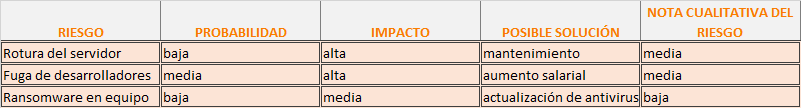
\includegraphics[width=6in]{matriz_de_riesgo.png}
  		   \caption{Matriz de riesgo.}
  		   \label{img:matriz_riesgo}
\end{figure}
\item {\bfseries Check-lists:}
Es una técnica que permite identificar los riesgos de una manera simple, proporcionando una lista de incertidumbres típicas a considerar.

\item {\bfseries SWIFT:}
Al igual que check-lists, sirve para identificar riesgos.
\item {\bfseries Análisis de árbol de fallas:}
Esta técnica se inicia viendo cómo se comporta algunos de los recursos del sistema de información ante un evento no deseado, y determina todas las maneras en las que este podría ocurrir, se representa gráficamente en un diagrama de árbol lógico.\\
Se muestra un ejemplo de esta herramienta en Figura \ref{img:diagrama_arbol_de_fallas} \cite{daf}.
\begin{figure}[tphb]
  		   \centering
     		   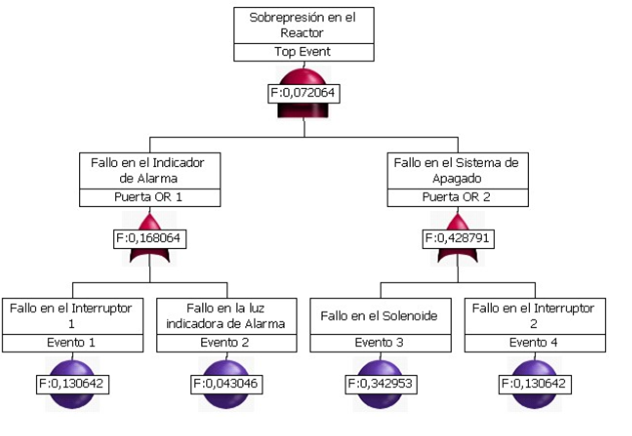
\includegraphics[width=6in]{diagrama-arbol-fallas.png}
  		   \caption{Diagrama árbol de fallas.}
  		   \label{img:diagrama_arbol_de_fallas}
\end{figure}
\item {\bfseries Diagrama causa-efecto:}
Esta herramienta permite conocer la raíz de un problema y cuellos de botella en procesos. Se representa mediante un diagrama denominado espina de pescado.\\
Se muestra un ejemplo de esta herramienta en Figura \ref{img:diagrama_causa_efecto} \cite{diagrama-pescado}.
\begin{figure}[tphb]
  		   \centering
     		   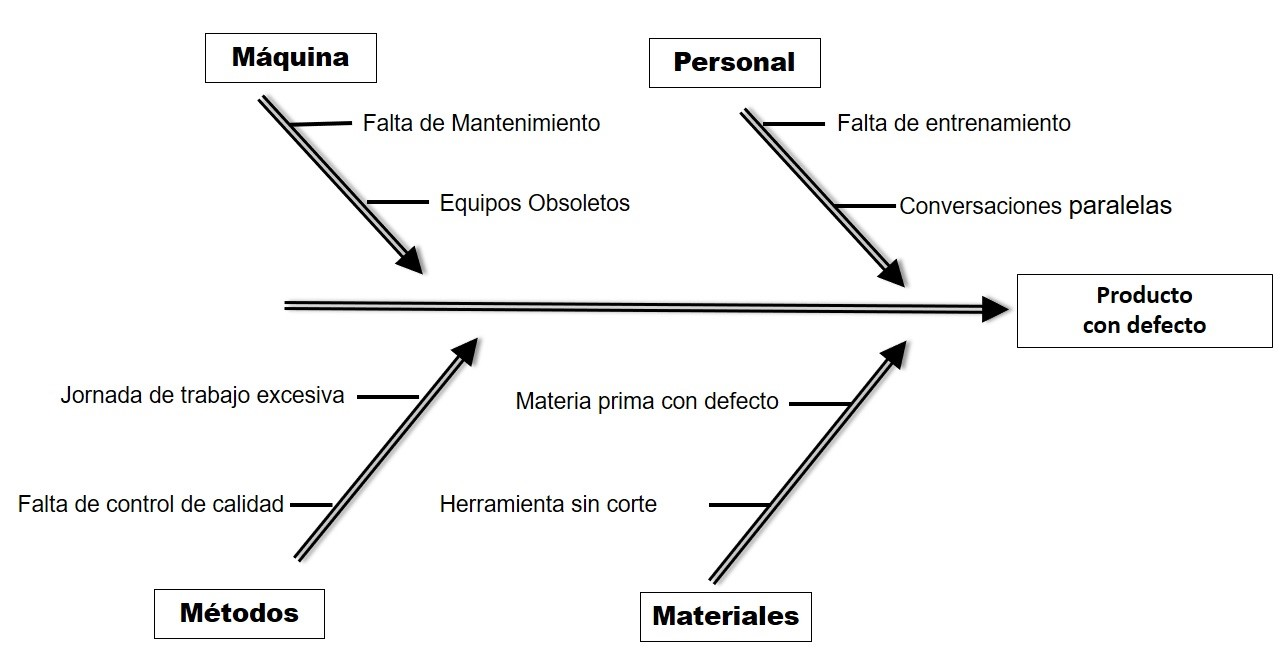
\includegraphics[width=6in]{diagrama-causa-efecto.jpg}
  		   \caption{Diagrama causa-efecto.}
  		   \label{img:diagrama_causa_efecto}
\end{figure}

\item {\bfseries AMFE:}
Esta técnica identifica y analiza los fallos potenciales, mecanismos y los efectos de esos fallos. \\
Se muestra un ejemplo de esta herramienta en Figura \ref{img:amfe} \cite{amfe}.
\begin{figure}[tphb]
  		   \centering
     		   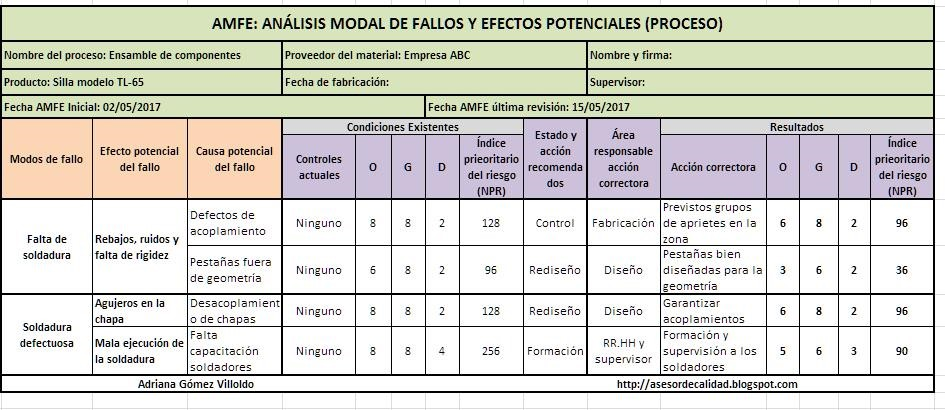
\includegraphics[width=7in]{AMFE.jpg}
  		   \caption{AMFE.jpg}
  		   \label{img:amfe}
\end{figure}

\item {\bfseries HAZOP:}
Esta herramienta tiene como objetivo detectar situaciones de inseguridad en plantas industriales, debido a la operación o a los procesos productivos.\\
Se muestra un ejemplo de esta herramienta en Figura \ref{img:hazop} \cite{hazop}.
\begin{figure}[tphb]
  		   \centering
     		   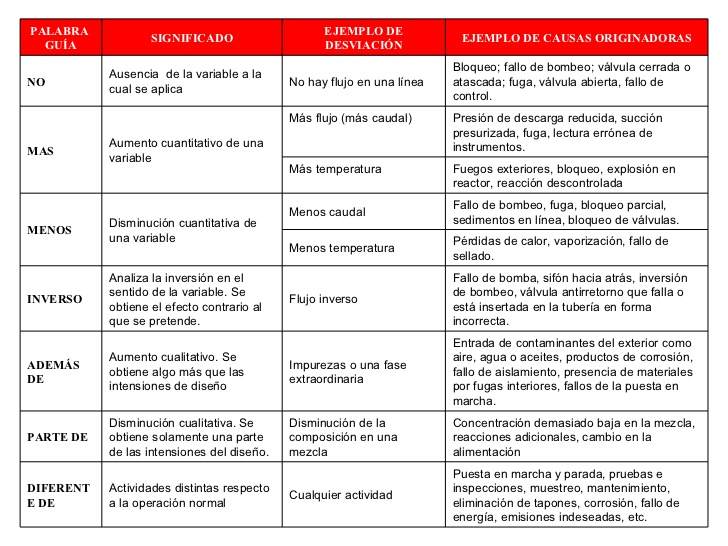
\includegraphics[width=6in]{hazop.jpg}
  		   \caption{HAZOP.}
  		   \label{img:hazop}
\end{figure}

\item {\bfseries LOPA:}
Permite la evaluación de controles, así como la determinación de su eficacia.\\
Se muestra un ejemplo de esta herramienta en Figura \ref{img:lopa} \cite{lopa}.
\begin{figure}[tphb]
  		   \centering
     		   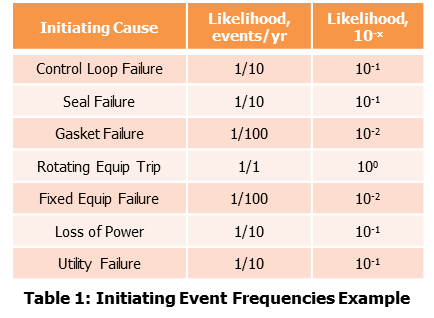
\includegraphics[width=2in]{LOPA.png}
  		   \caption{LOPA.}
  		   \label{img:lopa}
\end{figure}

\end{enumerate}




%-------------------------------------------PARTE 4-----------------------------------------------------------------------------------
\chapter{Ciberataques y sus consecuencias}
\label{cha:ciberataques-y-consecuencias}

Antes de conocer los distintos tipos de ciberataques y las consecuencias de los mismos, debemos definir que es un ciberataque. La Real Academia 
de la Ingeniería define ciberataque como:

\emph{"Forma de ciberguerra o ciberterrorismo donde, combinado con ataque físico o no, se intenta impedir el empleo de los sistemas de información 
del adversario o el acceso a la misma." \cite{ciberataque-rai}}.

Estos ciberataques aprovechan alguna de las vulnerabilidades ya comentadas en el capítulo \ref{cha:vulneravilidades-y-ataques}, para robar o destruir
no solo datos empresariales fundamentales, sino comprometer sitios web e interrumpir estructuras operativas, así como el robo de identidad de personas.

\begin{figure}[tphb]
  		   \centering
     		   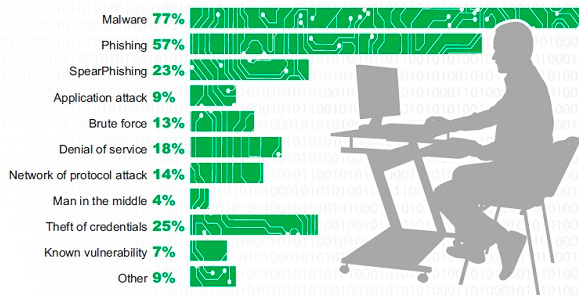
\includegraphics[width=5in]{ciberataques.png}
  		   \caption{Ciberataques mas comunes \cite{ciberataques}}
  		   \label{img:ciberataques}
\end{figure}

Tanto si el motivo es el espionaje como el sabotaje, los ciberdelincuentes emplean distintos métodos de ataque, algunos de ellos son el "spear-phishing",
 el ataque de inyección SQL, el filtro de scripts de sitios (XSS), los ataques de fuerza bruta... Una de las tácticas más perturbadora utilizada en los ciberataques 
es el ataque distribuido de denegación del servicio (DDoS), en el que se utilizan bots infectados para congestionar un sitio web o una aplicación web hasta el punto 
de que los usuarios legítimos no pueden acceder a él, algo que cuesta a las empresas millones de dólares en ingresos, pérdida de productividad y daños en la reputación.\nocite{akamai}
En este capitulo se mencionan algunos de los ciberataques mas conocidos, así como su funcionamiento y las consecuencias del mismo.

\section{Software malicioso: Malware}
\label{sec:malware}

La palabra malware viene del inglés, y es el resultado de la unión de las palabras malicious software(software malicioso). Se trata de un tipo de software o de aplicación que tiene como objetivo hacer daño al dispositivo en el que se ha conseguido alojar, instalar o infiltrar, ya sea un ordenador, un teléfono móvil… 
Existen muchos tipos de malware, los troyanos, los gusanos, el spyware, el ransomware. Sin embargo, malware es el término principal que se emplea para hablar de todas esas amenazas informáticas. La forma de actuar de cada uno suele ser diferente, pero en común tienen el objetivo de dañar el equipo o a su usuario. A continuación, se enumeran los tipos de malware más conocidos:

\begin{enumerate}

\item {\bfseries Virus informático:}
Este es un tipo de malware cuyo objetivo es alterar el correcto funcionamiento de un dispositivo. Un virus necesita ser ejecutado por el usuario pensando que es una aplicación legítima, y una vez lo hace, puede replicarse e infectar el equipo.

\item {\bfseries Gusano informático:}
A diferencia del virus informático, este malware no necesita de la intervención del usuario ni modificar ningún archivo existente. Se suelen utilizar para crear redes de ordenadores “zombies” que pueden actuar de forma simultánea para enviar SPAM de forma masiva, difundir malware o lanzar diferentes tipos de ataques informáticos.

\item {\bfseries Troyano:}
Este malware se oculta dentro de un programa legítimo o se disfraza de él para introducirse en un equipo como si de un Caballo de Troya se tratase. Mientras que un virus suele ser destructivo, un troyano trata de pasar desapercibido mientras accede a tu dispositivo con la intención de ejecutar acciones ocultas.

\item {\bfseries Spyware:}
Al igual que el troyano, spyware se instala en el equipo mediante la interacción de una segunda aplicación que lo lanza, trabaja en segundo plano intentando no ser detectado para recolectar información sobre el usuario u organización dueña de un ordenador de forma no autorizada.

\item {\bfseries Ransomware:}
Se trata de un tipo de malware que secuestra los datos de cualquier dispositivo electrónico, bloqueándolos y pidiendo un rescate económico a cambio de recuperarlos.

\nocite{malware}

\end{enumerate}


\section{Phishing y Spear-phishing}
\label{sec:phishing-spear-phishing}

El principio del phishing es relativamente sencillo, los estafadores crean correos electrónicos, páginas web e incluso mensajes cortos de carácter falso 
que solicitan información de inicio de sesión de los usuarios. Es así como los estafadores se hacen con los datos de acceso para tiendas online, redes 
sociales, espacios de almacenamiento en la nube y en el peor de los casos, se hacen incluso con información bancaria o datos de la tarjeta de crédito. 
De esta forma, con una página web de phishing sencilla se pueden obtener datos sensibles, información que tiene un alto valor económico en el mercado 
negro digital.

A partir de los correos electrónicos,  los ciberdelincuentes acaban consiguiendo datos de acceso y contraseñas. No obstante, hoy en día, las 
probabilidades de que los usuarios caigan en el engaño de los mensajes falsos son bastante reducidas. Ahora hay una nueva variante de este tipo de 
engaño, el spear-phishing, mucho más concreta y, por lo tanto más peligrosa.

\begin{figure}[tphb]
  		   \centering
     		   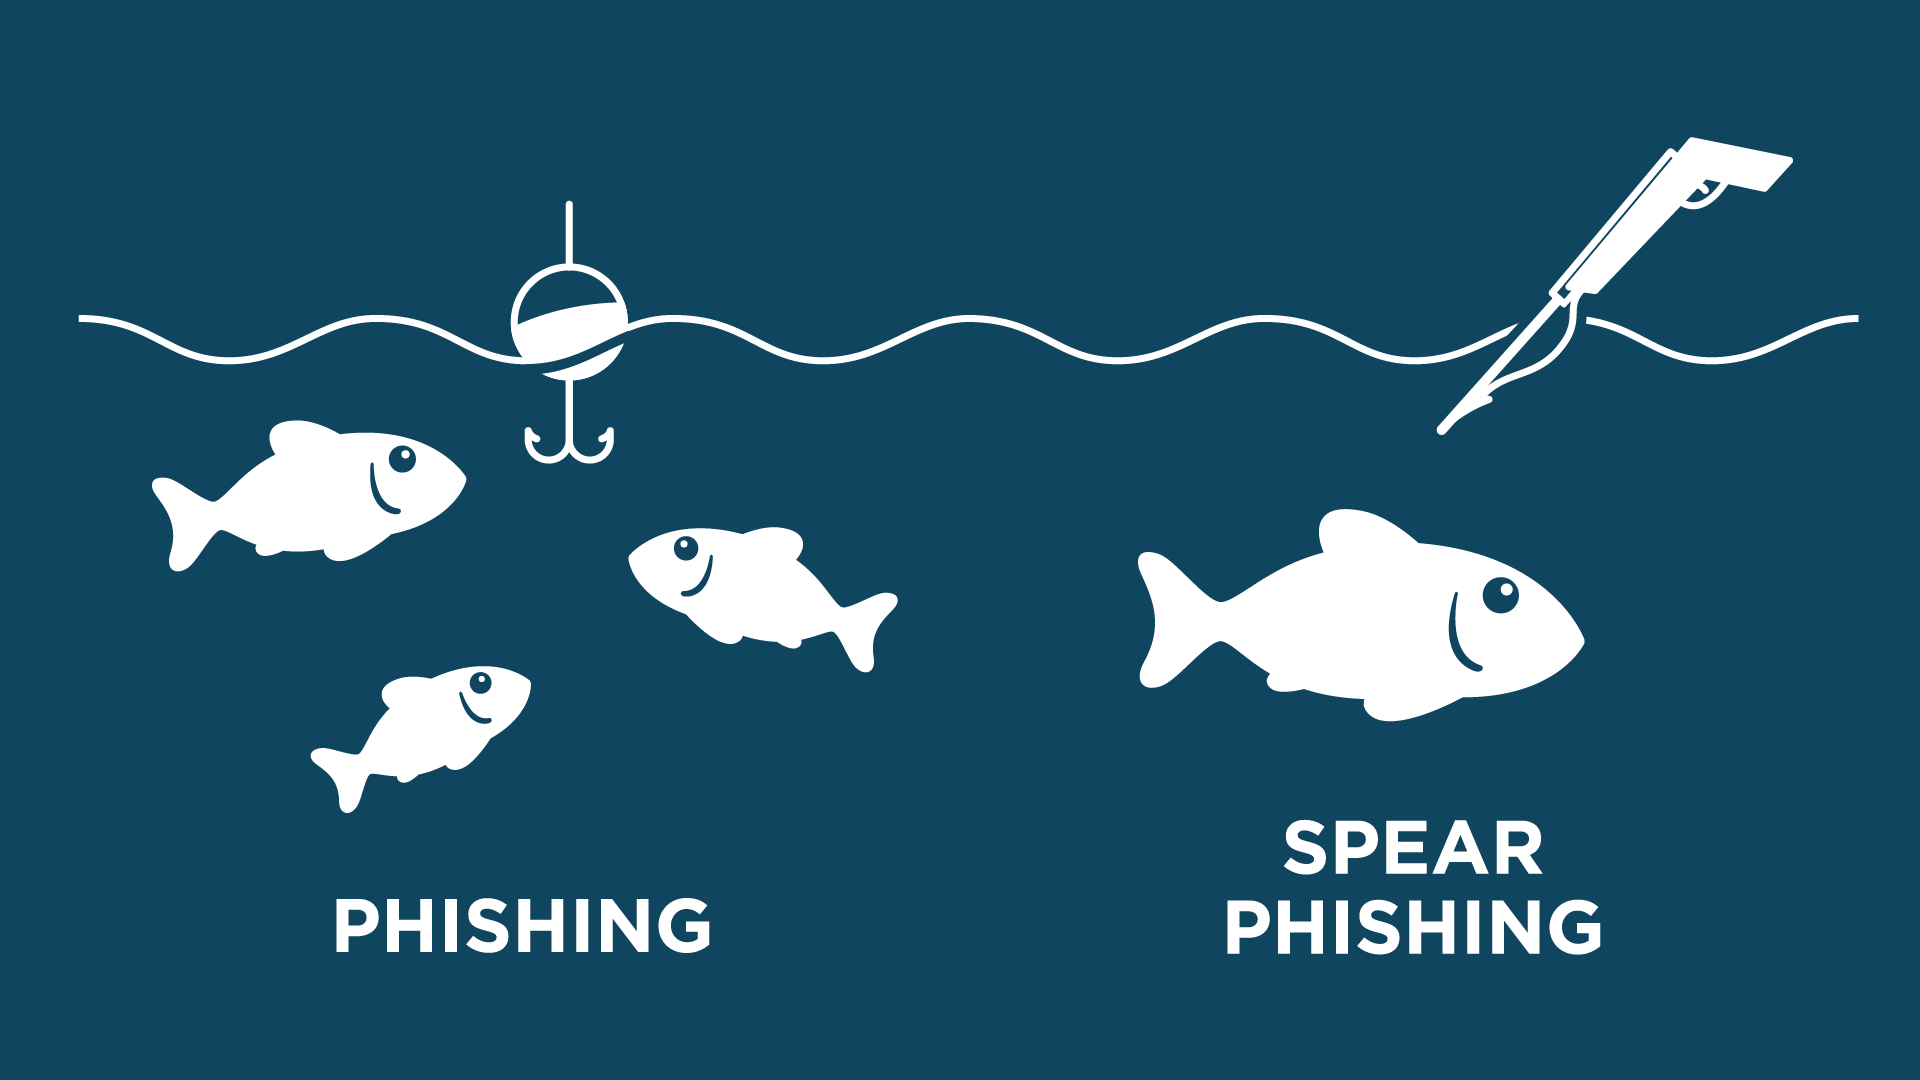
\includegraphics[width=5in]{spear-phishing.png}
  		   \caption{Pishing vs Spear-phishing \cite{armor}}
  		   \label{img:spear-pishing}
\end{figure}

El spear-phishing, a diferencia del phishing tradicional, es mucho más específico. En este caso, se selecciona a una víctima concreta y el engaño se adapta de forma precisa a la 
persona elegida. Por eso, el principal foco de estos ataques suelen ser empresas y organizaciones. Los agentes que emplean esta variante de phishing 
también suelen diferenciarse de los estafadores habituales. En lugar de recopilar todo tipo de información aleatoria para venderla al mejor postor, estos
ladrones actúan específicamente contra la víctima seleccionada para causar daño a la empresa o la organización afectada. Por ello, al margen del robo de 
datos bancarios, también se perpetúan crímenes de espionaje industrial y ciberataques sobre objetivos militares o la infraestructura de una región.

\section{SQL Injection}
\label{sec:sql-injection}

SQL Injection es uno de los Ciberataques más frecuentes y amenazadores, ya que puede atacar cualquier sitio web o aplicación que use una base de datos. 
El ataque consiste en usar un trozo de código para manipular una base de datos y acceder a información potencialmente valiosa empleando consultas SQL. 
Una consulta SQL no es mas que una solicitud enviada a una base de datos. 

Por ejemplo, la información de inicio de sesión de una página web se envía a través de un formulario antes de que el usuario pueda acceder al sitio. Normalmente, 
este tipo de formulario web está diseñado para aceptar solo tipos muy específicos de datos, como un nombre o una contraseña. Cuando se agrega esa información, 
esta se coteja contra una base de datos y, si coincide, se otorga acceso al usuario. De lo contrario, se deniega el acceso.

Los problemas surgen porque la mayoría de los formularios web no tienen forma de detener el ingreso de información adicional a través de consultas SQL. Así, los 
cibercriminales pueden aprovechar esta vulneravilidad y utilizar los cuadros de entrada del formulario para enviar sus propias solicitudes a la base de datos. Esto 
podría permitirles llevar a cabo una amplia gama de actividades maliciosas, desde el robo de datos confidenciales hasta la manipulación de la información de la base 
de datos para sus propios fines.

\begin{figure}[tphb]
  		   \centering
     		   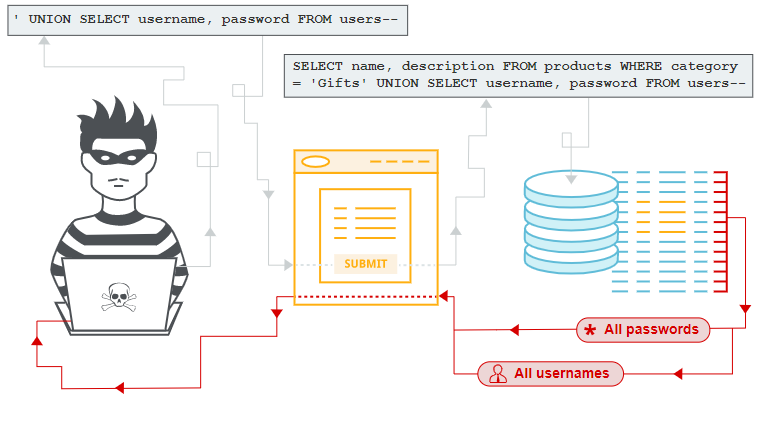
\includegraphics[width=5in]{sqli.png}
  		   \caption{SQL Injection \cite{sqli}}
  		   \label{img:sqli}
\end{figure}

Debido a la prevalencia de sitios web y servidores que utilizan bases de datos, el método de ataque de inyección SQL es uno de los tipos de ciberataques más antiguos 
y generalizados. Varios avances han aumentado el riesgo de este tipo de ataques, en especial la llegada de programas de inyecciones SQL automatizadas. Estos
programas permiten realizar ataques automáticamente en tan solo minutos, pudiendo acceder a cualquier tabla o columna de una base de datos con tan solo un clic 
y un proceso de ataque.

\section{Cross site scripting(XSS)}
\label{sec:Cross site scripting}
Como acabamos de ver en la sección anterior 4.3, el objetivo de los ataques por inyección de código SQL es obtener información de la base de datos de una empresa 
u organización. Los ataques por Cross site scriting tienen la misma finalidad que SQL Injection, obtener información a través de consultas SQL, pero en este caso el 
objetivo no son empresas ni organizaciones sino usuarios individuales.

La inyección de código, al igual que en el caso del SQL, consiste en intercalar pequeños programas o comandos en medio del texto que se escribe en ese recuadro, 
pero ahora no será el servidor web, ni el sistema de gestión de la base de datos quienes ejecutarán ese código, como en el caso del SQL Injection, sino que ahora 
con la vulnerabilidad XSS quien ejecutará ese código es el navegador del usuario víctima.

\begin{figure}[tphb]
  		   \centering
     		   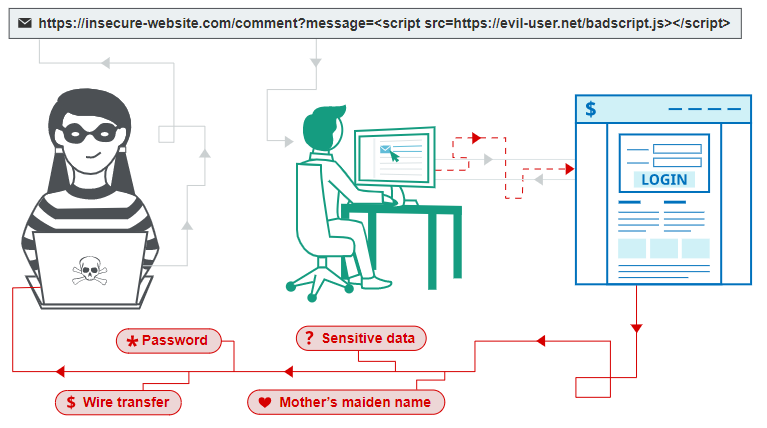
\includegraphics[width=5in]{xss.png}
  		   \caption{Cross site scripting \cite{xss}}
  		   \label{img:xss}
\end{figure}

\begin{enumerate}
\item {\bfseries Cross Site Scripting persistente:}
Si el código SQL insertado se queda almacenado en el servidor, formando parte de una aplicación web, se dice que el ataque es persistente. Normalmente el atacante
trata de insertar tags propios de HTML como <iframe>, o <script>, de esta forma el atacante podría ejecutar código malicioso.

\item {\bfseries Cross Site Scripting reflejado:}
Si el código que insertamos no se queda almacenado en la web, sino que va embebido dentro de un enlace que se hace llegar de algún modo a la víctima para que 
pinche en él, se dice que este tipo de ataque es reflejado. La característica diferencial con el anterior ataque es que en este caso en el servidor web no queda almacenado nada.

\end{enumerate}

\section{Ataque por denegación de servicio}
\label{sec:denegacion-servicio}

Un ataque de denegación de servicio tiene como objetivo inhabilitar el uso de un sistema, una aplicación o una máquina, con el fin de bloquear su servicio. Este ataque 
puede afectar, tanto a la fuente que ofrece la información como puede ser una aplicación o el canal de transmisión, como a la red informática. Existen dos técnicas de este tipo de ataques, la denegación de servicio o DoS (Denial of Service) y la denegación de servicio distribuido o DDoS (Destributed Denial of Service).

En los ataques DoS se generan una cantidad masiva de peticiones al servicio desde una misma máquina o dirección IP, consumiendo así los recursos que ofrece el servicio hasta que llega un momento en que no tiene capacidad de respuesta y comienza a rechazar peticiones, esto es cuando se materializa la denegación del servicio.

En el caso de los ataques DDoS, se realizan peticiones o conexiones empleando un gran número de ordenadores o direcciones IP. Estas peticiones se realizan todas al mismo tiempo y hacia el mismo servicio objeto del ataque. Un ataque DDoS es más difícil de detectar, ya que el número de peticiones proviene desde diferentes IP´s y el administrador no puede bloquear la IP que está realizando las peticiones, como sí ocurre en el ataque DoS.

\begin{figure}[tphb]
  		   \centering
     		   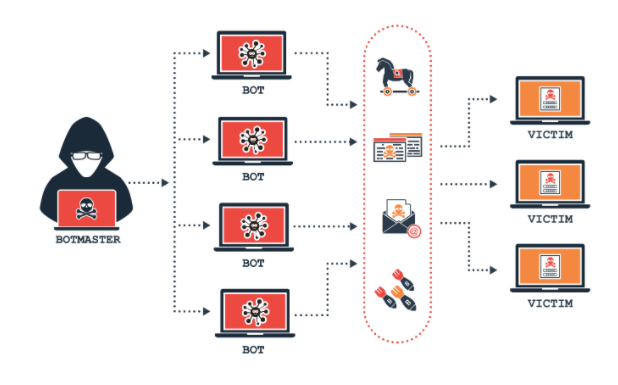
\includegraphics[width=5in]{ddos.png}
  		   \caption{Ataque por denegacion de servicio \cite{ddos}}
  		   \label{img:ddos}
\end{figure}

Como hemos visto, los ataques de denegación de servicio son utilizados para inhabilitar un servicio ofrecido por un servidor, haciendo colapsar el sistema aprovechando sus vulnerabilidades. El objetivo de los ciberdelincuentes es provocar un perjuicio, tanto a los usuarios que se abastecen del servicio, como al administrador que lo ofrece, inhabilitando su funcionalidad y provocando pérdidas, tanto económicas, como de prestigio



%-------------------------------------------PARTE 5------------------------------------------------------------------------------------
\chapter{Planificación de respuesta a incidentes}
\label{cha:planificacion-de-respuesta}

Mientras que las organizaciones durante estos últimos años han mejorado lentamente en su capacidad 
de detectar y responder a los ciberataque, su capacidad de contener un ataque ha disminuido en un 
13\% durante este mismo período según un estudio realizado por Cyber Resilient Organization Report.\cite{ibm-article}

Según la encuesta, los esfuerzos en materia de seguridad se vieron obstaculizados por el uso de 
demasiadas herramientas, así como por la falta de planes estratégicos específicos para los tipos de 
ataque más comunes. Aunque la planificación para la respuesta de seguridad está mejorando poco a 
poco, la gran mayoría de las organizaciones carecen de una guía concreta con los pasos a seguir.

Un plan de respuesta a incidentes cibernéticos consiste en un documento que incluye un conjunto 
de instrucciones diseñadas para ayudar a las empresas a detectar, responder y recuperarse de los 
incidentes de seguridad de la red. La mayoría de estos planes se centran en la tecnología y abordan 
problemas como la detección de malware, el robo de datos y las interrupciones del servicio. Sin 
embargo, cualquier ataque cibernético ya sea alguno de los mencionados en el Capítulo 
\ref{cha:ciberataques-y-consecuencias} o cualquier otro, puede afectar a una organización a través 
de sus funciones de múltiples maneras.

Una vez que tenemos clara la necesidad de contar con un plan de respuesta ante ciberataques, el 
siguiente paso es el de definir los distintos puntos que debe contemplar dicho documento, que ha de 
ser lo más completo posible para abarcar todas las situaciones que puedan suceder. Existen una serie 
de puntos que deben ser analizados en un plan de esta índole:

\begin{enumerate}

\item {\bfseries Auditoría e identificación de la amenaza:}
El primer punto del plan de respuesta ante ciberataques debe ser el que especifique los mecanismos 
necesarios para identificar correctamente la amenaza, incluyendo tanto los procesos internos como
la gestión de fuentes de información externas. En este primer punto también debe analizarse y 
valorarse si la amenaza es real o no, así como qué nivel de gravedad representa para la organización.

\item {\bfseries Comunicación y notificación:}
Una vez detectado el incidente, el plan debe recoger el procedimiento para notificar lo más rápido 
posible el problema a todos los individuos implicados en el equipo de respuesta.

\item {\bfseries Equipo de respuesta:}
Para poder enviar estas notificaciones y responder al cibercriminal, debe existir un equipo de respuesta 
perfectamente organizado, con responsabilidades bien definidas, preparado y disponible las 24 horas 
para atender esta necesidad.

\item {\bfseries Comunicación externa:}
En la línea anteriormente mencionada, el plan de respuesta ante ciberataques debe recoger cómo se 
afrontará esa crisis de forma pública, tanto ante los medios de comunicación como en redes sociales 
y también ante los organismos oficiales correspondientes.

\item {\bfseries Comunicación externa:}
El aspecto central del plan es la metodología y las tecnologías que serán utilizadas para eliminar la 
amenaza, reducir el impacto sobre el negocio y acabar con el problema en todas sus vertientes.

\item {\bfseries Evaluación final y desactivación del plan:}
Una vez que se haya desactivado el virus, el equipo de respuesta debe evaluar de nuevo la situación 
para decidir si ha llegado el momento de desactivar ‘el estado de alarma’. Además, también es un buen 
momento para asimilar lo aprendido durante el episodio y modificar los métodos preventivos y sistemas 
de respuesta de forma que se evite cualquier réplica futura de la amenaza.

\end{enumerate}



%-------------------------------------------PARTE 6------------------------------------------------------------------------------------
\chapter{Protección informática}
\label{cha:proteccion-informatica}
La protección informática consiste en el área que se encarga de proteger la información que se encuentra localizada en un sistema.
\section{Caraterísticas de la protección informática}
Las cinco características que garantizan una buena protección informática son:
\begin{enumerate}
\item {\bfseries Autentificación:}
Permite verificar que la identidad del propietario de un archivo mediante una referenciación en dicho documento. Esta cualidad genera que se pueda corroborar si alguien es quien dice ser, un ejemplo de este mecanismo es la autentificación mediante usuario y contraseña.
\item {\bfseries Integridad:}
Hace alusión a que la información no haya sido modifica y esté totalmente correcta sin que se hayan borrado o editado datos desde que fueron generados. Esto se logra mediante la generación de un hash, que se trata de la generación de un texto corto a partir del archivo original mediante funciones matemáticas. Si se compara el hash del archivo original con la del archivo actual y son iguales, significa que archivo sigue integro y no fue modificado, sin embargo, si son distintas implica que el archivo fue modificado.
\item {\bfseries Confidencialidad:}
Esta cualidad permite que los datos no sean accesibles a sistemas y personas no deseadas, haciendo que los datos estén cifrados y solo puedan ser legibles para las personas o sistemas autorizados. En el caso de que una persona no autorizada intercepte la información esta lo verá de una forma ilegible debido a que los datos estarán encriptados, esta cualidad se puede implementar mediante criptografía simétrica o asimétrica, en la criptografía simétrica tanto solo el emisor y receptor conocen una clave para desencriptar el archivo. Con la criptografía asimétrica el emisor tiene una clave privada que solo conoce el mismo y una clave pública ligada a la privada que conoce todo el mundo, el emisor encriptará los datos con su clave privada y el receptor los desencriptará con la clave pública del emisor.
\item {\bfseries Disponibilidad:}
Como su nombre indica esta cualidad permite el acceso y la utilización cuando y donde sea de los servicios a través de un canal seguro. También se incluye que información eliminada sea recuperable en todo momento pudiendo evitar su pérdida o bloqueo. Esta característica es de las más importantes para las grandes empresas como Facebook y en hospitales y aeropuertos debido a que necesitan que sus servicios estén funcionando las 24 horas los 7 días de la semana.
\item {\bfseries No repudio:}
Consiste en la irrenunciabilidad por parte de la información de un emisor. Es muy similar a la autentificación, sin embargo, se diferencia en que la autentificación se centra en las personas implicadas y la cualidad de no repudio va enfocada frente a terceros. Un ejemplo de esta característica serían las firmas electrónicas, el proceso es bastante similar al de la criptografía simétrica usado en la confidencialidad, una persona crea un documento del que se obtiene el hash, este hash es encriptado con la clave privada dicha persona y el resultado de esto es la firma electrónica que es añadida al documento.
\end{enumerate}



%-------------------------------------------PARTE 7------------------------------------------------------------------------------------
\chapter{Sistemas utilizados para mantener la seguridad y la privacidad}
\label{cha:tipos-sistemas}
\section{Sistemas hardware}
Consiste en aplicar impedimentos físicos y funciones de control como medida de prevención y contra medidas ante amenazas a recursos confidenciales, estos procedimientos son aplicados en equipos del hogar, oficinas y a servidores y cpds. Los principales sistemas hardware mas utilizados para garantizar la seguridad son:
\begin{enumerate}
\item {\bfseries RAID (Redundant Array of Independent Disk):}
Es usado para crear un único volumen lógico, el cual físicamente esté compuesto por varios discos físicos. Dependiendo de qué modo de RAID utilicemos, esto nos servirá para conseguir un volumen con mayor seguridad contra fallos de hardware de los discos que lo componen gracias al almacenamiento redundante de estos o para conseguir simplemente un volumen de capacidad mayor. Los modos de raid que ofrecen una mayor seguridad del dispositivo son:
\begin{enumerate}
\item {\bfseries RAID 1:}
Para ello son necesarios al menos 2 discos de igual tamaño, se realiza una copia espejo es decir lo que de escribe en uno se copia en el otro permitiendo de esta forma que, aunque se produzca un fallo en uno de los 2 discos sigamos conservando la información en otro el disco.
\item {\bfseries RAID 5:}
En esta configuración necesitaremos mínimo 3 discos de la misma capacidad, la capacidad total de almacenamiento será la de todos los discos menos uno, es decir, dos y los datos se irán almacenando de forma parcialmente redundante permitiendo que, aunque suframos un fallo en uno de los discos, podamos seguir accediendo a toda la información. Este sistema es más eficiente que el RAID 1 debido a que en este solo tenemos la capacidad de almacenamiento de uno de los discos y en el RAID 5 tenemos la capacidad de dos, aunque la desventaja de este sistema es que requiere un disco más.
\end{enumerate}
\item {\bfseries Sistemas de Alimentación Ininterrumpida (SAI):}
Son dispositivos que ofrecen protección contra apagones o irregularidades en la corriente eléctrica. Su principal función es suministrar la energía eléctrica que tienen acumuladas en sus baterías cuando se producen cortes eléctricos evitando así posibles fallos y averías en los sistemas conectados el evitan que se apaguen de forma repentina, además algunos SAI poseen un regulador de tensión que asegura estabilidad en la corriente logrando una alimentación de los dispositivos conectados más constante y así prolongando la vida útil de dichos sistemas.
\item {\bfseries Firewall de hardware:}

También conocido como cortafuegos se trata de un dispositivo que es capaz de bloquear comunicaciones no autorizadas, permitiendo las que si lo están. Los cortafuegos permiten una configuración para permitir y limitar el tráfico entre distintas redes o ámbitos de una red mediante un conjunto de reglas y normas. Sus principales características son el filtrado por aplicación, reglas de filtrado sobre el tráfico de entrada y salida de una red en una interfaz de red, filtrado de paquetes comprobando su MAC, IP o puerto destino y origen y almacenar el registro del filtrado de paquetes. También existe el firewall de software, la diferencia es que el cortafuegos de hardware se trata de un dispositivo dedicado únicamente como firewall y el de software no. Las arquitecturas de cortafuegos más implementadas son:
\begin{enumerate}
\item {\bfseries Screening router:}
 Un router hace de frontera entre la red pública y la red privada, realizando la función de cortafuegos.
\item {\bfseries Dual Homed-Host:}
Un servidor con al menos dos interfaces de red divide la red pública de la red privada y la función de firewall.
\item {\bfseries Screened Host:}
Se trata de la combinación de un router como frontera y un servidor proxy que realizará las tareas de filtrado.
\item {\bfseries Screened-subnet:}
Se crea una red intermedia entre la red externa y la red privada denominada DMZ o zona desmilitarizada en la que se localizan los servidores, teniendo un nivel de seguridad mayor en el cortafuegos de acceso a la red interna y uno menor en el cortafuegos hacia la red externa.
\end{enumerate}
\item {\bfseries Servidor proxy:}
Consiste en un sistema que gestiona conexiones de red, haciendo de intermediario entre las peticiones de los servidores y los clientes, como FTP, DNS, https, etc., generando de tal forma una memoria caché con las diversas peticiones y respuestas de los servidores. Aunque su principal finalidad no es la seguridad sino que es servir más rápidamente a las conexiones siguientes que hayan sido solicitadas, añade funciones de autentificación y control de usuarios, reglas de filtrado de contenidos solicitados y un registro de logs. Los tipos de servidor proxy que ofrecen una mayor seguridad son:
\begin{enumerate}
\item {\bfseries Proxy transparente:}
Para el uso de este servidor proxy es necesario la configuración de cada cliente manualmente. Se encarga de redireccionar todas las conexiones al puerto 80 (http) hacia el puerto del servidor haciendo que estas conexiones sean más seguras.
\item {\bfseries Proxy anónimo:} 
Este servidor proxy aumenta la privacidad y el anonimato de los clientes mediante una eliminación activa de característica identificativas como la dirección IP del cliente, cookies, identificadores de sesión, etc.
\item {\bfseries Proxy caché web:}

-Proxy caché Web: Este proxy es usado específicamente para web y se encarga de hacer copias locales de los archivos más solicitados por los clientes.
\item {\bfseries Proxy inverso:}
 Consiste en un servidor proxy instalado en una red con varios servidores web y realizará en función de intermediario a las peticiones externas ofreciendo una capa de seguridad previa, además de distribuir la carga de las distintas peticiones externan y gestionar el SSL.
\end{enumerate}
\end{enumerate}








% fin del trabajo
\nocite{ransomware}
\nocite{sql_injection}
\nocite{vulnerabilidades}
\nocite{vulnerabilidades2}
\nocite{wikip}
\nocite{comision_europea}
\nocite{isot}
\nocite{gestion_activos}
\nocite{incibe2}
\nocite{herramientas-evaluacion-riesgos}
\nocite{bibdigital}
\nocite{bibdigital}

\nocite{xss2}
\nocite{pri}

%se incluye el archivo de biobliografia
%%%%%%%%%%%%%%%%%%%%%%%%%%%%%%%%%%%%%%%%%%%%%%%%%%%%%%%%%%%%%%%%%%%%%%%%%%%
%
% Generic template for TFC/TFM/TFG/Tesis
%
% $Id: bibliography.tex,v 1.9 2015/06/05 00:10:32 macias Exp $
%
% By:
%  + Javier Macías-Guarasa. 
%    Departamento de Electrónica
%    Universidad de Alcalá
%  + Roberto Barra-Chicote. 
%    Departamento de Ingeniería Electrónica
%    Universidad Politécnica de Madrid   
% 
% Based on original sources by Roberto Barra, Manuel Ocaña, Jesús Nuevo,
% Pedro Revenga, Fernando Herránz and Noelia Hernández. Thanks a lot to
% all of them, and to the many anonymous contributors found (thanks to
% google) that provided help in setting all this up.
%
% See also the additionalContributors.txt file to check the name of
% additional contributors to this work.
%
% If you think you can add pieces of relevant/useful examples,
% improvements, please contact us at (macias@depeca.uah.es)
%
% You can freely use this template and please contribute with
% comments or suggestions!!!
%
%%%%%%%%%%%%%%%%%%%%%%%%%%%%%%%%%%%%%%%%%%%%%%%%%%%%%%%%%%%%%%%%%%%%%%%%%%%

%\bibliographystyle{plainnat}
%\bibliographystyle{dinat}
%\bibliographystyle{unsrt}
\bibliographystyle{IEEEtran}

% The following is overly complicated because I was not able to do so in
% another way. The problem is the bibliography command being "called"
% from both the root and anteproyecto directories...
%
% Here define as many bibfiles as needed
\newcommand{\mybibfileOne}{biblio/biblio}
\newcommand{\mybibfileTwo}{biblio/biblio2}
%...
%\newcommand{\mybibfileN}{biblio/biblioN}

% This is for a single bib file
\newcommand{\mybibfiles}{\myreferencespath\mybibfileOne}
% but do this for multiple files
%\newcommand{\mybibfiles}{\myreferencespath\mybibfile1,\myreferencespath\mybibfile2,...,\myreferencespath\mybibfileN}

% Do not touch this
\inputencoding{latin1}
\bibliography{\mybibfiles}
\inputencoding{utf8}

%%% Local Variables:
%%% TeX-master: "../book"
%%% End:




\end{document}

